 %1-2 paragraph overview of science goals.  BAO, RSD, other applications.
 %SDT2015 as starting point.


%\begin{tcolorbox}[width=\textwidth,colback={mypink3},title={With true corners},outer arc=0mm,colupper=white]
%     Test
%     %%\includegraphics[scale=0.5]{frogimage.png}
%\end{tcolorbox}

\begin{tcolorbox}[width=\textwidth,colback={coralpink},outer arc=0mm,colupper=white]
     Test
     %%\includegraphics[scale=0.5]{frogimage.png}
\end{tcolorbox}



 \subsection{Requirements (D1)}

 The most important task of the SIT in guiding development of the WFIRST HLS
 spectroscopy is to set and validate the requirements of the instrument, the data
 reduction software, and the survey.  Accordingly, we have made this task our main focus
 over the past year. Our SIT made three deliveries of updates to
 the WFIRST GRS requirements to the WFIRST Project on July 1, 2016, December 1,
 2016, and March 2, 2017. These provide progressively precise definitions of the
 GRS requirements. We describe the main requirements and their science drivers
 below. This work was carried out by Wang, Eifler, Hirata, Ho, Kiessling, Krause, Merson, Padmanabhan, Pearson, Samushia,
 Benson, Capak, Dor\'e, Heitmann, Spergel, Teplitz, and Weinberg.

 \subsubsection{Science Requirements (Level 2a)}

 \noindent
 {\bf HLSS 1: The area to be surveyed shall be $\sim$1500 deg$^2$ (2000 deg$^2$ goal) after
 correcting for edge effects.  This area will be contiguous to the extent
 practical, and at least 90\% of the survey area must also be covered by the high
 latitude imaging survey. }

 The survey area should be contiguous and large enough to reduce edge effects in
 the BAO/RSD measurements.  The $>90\%$ overlap with the HLIS enables joint
 analysis of 90\% of WL and GRS data, which maximizes the dark energy science
 from WFIRST.  Imaging also provides undispersed galaxy positions, improving
 redshift determination.  The statistical precision of the dark energy
 constraints is sensitive to the survey area as well as the survey depth; a trade
 study of depth versus area will need to be carried out to optimize both, in the
 context of Euclid and LSST. We also need to investigate the impact of dividing
 the area into two equal patches near the NEP and SEP respectively, to take
 advantage of potential ground-based telescope resources.  A survey of one or
 two large, contiguous areas has smaller edge effects and better window functions
 than a survey comprised of many smaller areas.

 We have carried out trade studies of the HLSS survey design. We note that it
 will be important to conducting these trade studies in the context of the joint
 science return of HLSS and HLIS that properly accounts for correlations among
 spectroscopic and imaging observables and accounts for their correlated
 systematics.  We are in the progress of implementing a corresponding forecasting
 effort.  Here, we have carried out a trade study of area versus depth for the
 HLSS only, starting from a baseline survey of 2227 deg$^2$ and a wavelength
 range of 1.05-1.85 microns. We consider two alternative scenarios, i.e. a survey
 twice as wide and shallower and a survey half as wide but correspondingly
 deeper.  The galaxy redshift distributions were computed using the WFIRST
 Exposure Time Calculator ETC v14. The H$\alpha$ forecasts are based on the average
 of the 3 models in Pozzetti et al. (2016), and the [O III] forecasts are based
 on the Mehta et al.  (2015) luminosity function.
 %The resulting redshift distributions are shown in Fig. 1.
 We extend the CosmoLike framework (Eifler et
 al 2014, Krause \& Eifler 2016) to compute the constraining power of all scenarios
 on cosmic acceleration, closely following Wang et al (2013). We run 500,000 step
 MCMC simulated likelihood analysis in a 23 dimensional parameter space. We
 simultaneously vary 7 cosmological parameters and 16 ``nuisance'' parameters
 describing uncertainties due to the linear galaxy bias model, the non-linear
 smearing of the BAO feature, peculiar velocity dispersion, power spectrum shot
 noise, and redshift errors. We assume priors on cosmological parameters from the
 current state of the art experiments, i.e. the Planck mission, the Baryon
 Oscillation Spectroscopic Survey (BOSS), the Joint Lightcurve Analysis (JLA)
 supernovae, as described in Aubourg et al (2015).

 The information gain is quantified using the standard Dark Energy Task Force FOM
 and an extended cosmology FOM, which measures the enclosed volume in the full
 7-dimensional cosmological parameter space, not just in the 2 dark energy
 parameters. We will refer to these FOMs as DE-FOM and Cosmo-FOM.  Compared to
 the baseline survey, we find a decreased DE-FOM of 32\% and a decreased
 Cosmo-FOM of 45\% for the shallow/large area survey. For the deep/small area
 survey we find an increased DE-FOM of 5\% and an increased Cosmo-FOM of 2\%.
 While our trade study validates the design of the baseline survey, we note that
 these findings are model and prior dependent and will carry out further studies
 varying the input parameters. In particular, the [OIII] galaxy number density
 will be updated pending inclusion of the results from the latest observational
 data from HST grism observations.

 %LS edited this paragraph. Added more detail.
 We also investigated whether the survey area needs to be contiguous. We
 constructed two identical sets of Gaussian simulations one set covering
 contiguous 2000 deg$^2$ and a second set consisting of two $1000$ deg$^2$
 disjoint fields. The BAO signal was then measured in the 2D power spectrum using the
 most recent techniques applied to the BOSS DR12 data. The BAO positions measured
 in disjoint fields were biased by 1\% on average compared to the contiguous
 field in both line-of-sight and transverse directions. This bias persists even
 after properly correcting for the window effects and is unlikely to be coming
 from the sample variance since our sets consisted of close to one thousand
 independent simulations. This bias could be a result of either bigger than the
 box-size modes or various edge effects. The window of the real data will be more
 involved than we considered in our test case and the biases may be larger. This
 investigation is ongoing but our preliminary results seem to support the
 conclusion that a contiguous area is preferable for the standard BAO analysis.

  \noindent
 {\bf HLSS 2: The comoving density of galaxies with measured redshifts shall satisfy $n
 > 3\times10^{4}\ (h/\textrm{Mpc})^3$ at z=1.6. }

 This is set by $nP_{0.2} \sim1$ at $z=1.6$, with 20\% margin. Requiring $nP_{0.2}
 \sim1$ implies $n> 3\times10^{-4}\ (h/\mathrm{Mpc})^{-3}$ at $z=1.3$, and $n >
 6.5\times �10^{-4} (h/\mathrm{Mpc})^{-3}$ at $z=1.8$. Given the Hirata
 forecast of H$\alpha$ ELG counts (Model 3 in Pozzetti et al. 2016), $nP_{0.2}\sim0.6$ at $z=1.8$,
 and $nP_{0.2}>2$ at $z=1.3$.  We cannot require a higher galaxy number density than
 what nature provides, given fixed observing time and area coverage. Here we have
 chosen a characteristic high redshift, $z=1.6$, at which it is impossible for a
 ground-based survey to obtain spectra for a large number of galaxies. There
 remain large uncertainties in the H$\alpha$ LF due to the limited availability of
 uniform data. It is likely that the actual number of H$\alpha$ ELGs is higher than
 assumed here; thus we have additional margins for this requirement. We have
 assumed a bias for H$\alpha$ ELGs of $b(z) = 1+0.5z$. The bias relation has been rescaled
 to agree with Geach et al. (2012) measurement of $b=2.4$ at $z=2.23$ for $f >
 5\times 10^{-17} \, \mathrm{ erg\,s^{-1}cm^{-2}}$.

 This is significantly deeper than the Euclid GRS survey, which ensures that the
 WFIRST GRS is deep enough for carrying out robust modeling of systematic effects
 for BAO/RSD, higher order statistics, and the combination of weak lensing and
 RSD as tests of GR. This number density requirement could in principle be met
 using either H$\alpha$ or [OIII] ELGs, depending on the survey strategy. There is no
 need to set a separate requirement for [OIII] ELGs; this depth ensures high
 number densities for both [OIII] and H$\alpha$ ELGs.

 Galaxy number density is a key input in the dark energy Figure-of-Merit. It
 is very sensitive to the H$\alpha$ LF, which still has large uncertainties but will
 become better determined as more data become available and more comprehensive
 analyses are done. The flow down of the galaxy number density requirement here
 to the minimum survey depth depends on the LF of ELGs.
 Co-I Teplitz is a key member of the WISP team. He is supervising a postdoc, Ivano Baronchelli,
 in deriving more precise LFs for H$\alpha$ and [OIII] ELGs using WISP data.


 \noindent
 {\bf HLSS 3: The wavelength range of the HLSS will allow measurement of H$\alpha$ emission
 line redshifts over the redshift range $1.1 < z < 1.9$.}

 The corresponding wavelength range is 1.38 $\mu$m to 1.9 $\mu$m.  This wavelength
 coverage also allows measurements of [OIII] emission line redshifts over the
 range $1.8 < z < 2.8$.  A wider wavelength range that allows H$\alpha$ emission line
 detection over a wider redshift range is desirable, as it increases the survey
 volume and therefore adds margin for meeting other baseline requirements.  It is
 also critical that the WFIRST GRS redshift range is complementary to that of
 Euclid, with its red cutoff at 1.85 $\mu$m, or $z < 1.8$.

 The key consideration is that a space mission should focus on what cannot be
 accomplished from the ground, and be complementary to other space missions in
 wavelength coverage. Ground-based GRS can reach $z\sim1$ without great difficulty,
 thus we should focus on $z>1$. Euclid GRS can only reach $z \sim2$; its shallow depth
 does not enable a high enough number density of observed [OIII] ELGs. WFIRST GRS
 is deep enough to observe both H$\alpha$ (656.3nm) and [OIII] (500nm) ELGs, with the
 number density of the latter sensitive to the survey depth (the deeper the
 survey the higher their number density).

 For the nominal wavelength range of 1-2 microns, WFIRST GRS covers $0.52 < z <
 2$ using H$\alpha$ ELGs, and $1 < z < 3$ using [OIII] ELGs. Thus the redshift range
 requirement is met including both types of ELGs.

 In addition to the trade studies in HLSS 1 we examine the impact of an extended
 wavelength range on the DE-FOM and the Cosmo-FOM. We follow the same methodology
 as detailed in the HLSS 1 description in extending the wavelength range from
 1.05-1.85 microns for the baseline model to 1.00-1.89 for the extended model.
 %The corresponding redshift distributions of the galaxy samples computed from the
 %ETC v1.14 are shown in Fig. 2.
 We find a decreased DE-FOM of 2\% and a decreased
 Cosmo-FOM of 11\% for the extended wavelength survey with respect to our
 baseline scenario. While the FoM trade study seems to favor a narrower redshift
 range, we emphasize that these findings are model and prior dependent and will
 conduct further studies varying the input parameters. The reduction in the
 telescope temperature to 260K will have a major impact on this trade study. In
 addition, the FoM comparison is quantitative but simplistic; it does not reflect
 how the various future surveys will complement each other. Euclid GRS covers the
 wavelength range of 0.92-1.85 microns using the same BAO/RSD tracers as WFIRST,
 thus there is unique scientific value in WFIRST having a wavelength cutoff
 longer than 1.85 microns.


 \noindent
 {\bf HLSS 4: Redshift measurement errors $\sigma_z$ shall satisfy $\sigma_z <
 0.001(1+z)$, excluding outliers, for galaxies smaller than $0.54''$ in radius. The
 fraction of outliers with $|z_\mathrm{obs}-
 z_\mathrm{true}|/(1+z_\mathrm{true})>0.003$ shall be less than 10\%.}

 This is a requirement on the rms error of the redshift measurements, and not on
 every redshift measurement.

 We justify the requirement on the knowledge of the outlier fraction as follows.
 If you add a contaminant to the galaxy power spectrum with contamination
 fraction $\alpha$, then you leak in an amount of power from the ``wrong" line with
 amplitude $\alpha^2$, but you dilute the power spectrum of the ``real" signal by a factor
 of $(1-\alpha)^2$. For BAO the dilution is a minor issue (it reduces S/N), but for RSD
 it is a problem because it reduces the galaxy bias by $(1-\alpha)$ without changing the
 linear redshift-space distortion parameter $f\sigma_8$. So
 your inferred rate of growth of structure $f\sigma_8(z)$ is reduced by a factor
 of $1-\alpha$.  This leads to a stringent requirement on knowledge of $\alpha$ -- if it
 is 9.8\% but you think it is 10\% you have a 0.2\% systematic error, which is a
 reasonable budget for this contribution.

 Larger size galaxies have larger redshift errors. To assess redshift accuracy, a
 realistic pixel level grism simulation covering at least 2 square degrees needs
 to be carried out and processed. The current data from the HST grism survey WISP
 finds that 90\% of galaxies that would be observed by WFIRST (H$\alpha$ flux $>
 10^{-16} \mathrm{erg/s/cm}^2$, $0.55 < z < 1.85$) have a size less than $0.54''$
 (semi-major axis continuum size). Since the maximum redshift of the WISP sample
 is $\sim1.6$, WFIRST H$\alpha$ ELGs will likely have smaller sizes on average,
 see Figure \ref{fig:size_zbin}.

 The [OIII] ELGs are more compact, so this requirement is also sufficient for the
 redshift precision for [OIII] ELGs.

 \begin{figure}
 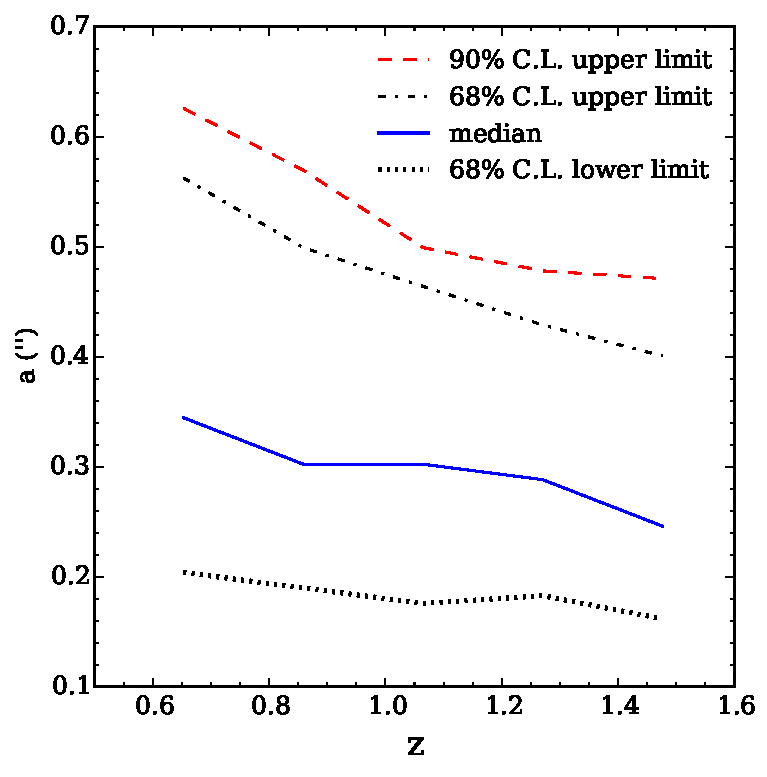
\includegraphics[width = 3.5in]{Plots/size_zbin.pdf}
 \label{fig:size_zbin}
 %\vspace{-1.25cm}
 \caption{\footnotesize{The 90\% upper limit of the semi-major axis continuum size of H$\alpha$ galaxies
 with H$\alpha$ line flux $>10^{-16} \mathrm{erg/s/cm}^2$, $0.55 < z < 1.85$), based on 1773 galaxies from
 WISP (WISP team, private communication).
 }}
 %\begin{center}
 %\end{boxedminipage}
 \end{figure}



 \noindent
 {\bf HLSS 5: Relative position measurement uncertainties shall be less than $3.4''$ over
 the entire survey area. }

 We need to measure galaxy positions to better than $\sim0.1 \mathrm{Mpc}/h$ (which corresponds
 to $3.4''$, assuming that 105 $\mathrm{Mpc/h}$ subtends 1 degree), in order to measure galaxy
 clustering accurately. This should be met easily if HLIS 26 is met, which makes
 systematic errors in the astrometry negligible. Given the pixel scale of
 $0.11''$, this requirement is automatically met within each field, and is tied to the
 precision of astrometry across different fields.


 \noindent
 {\bf HLSS 6: The survey completeness shall be 50\% (TBC), and the redshift purity
 shall be 90\% (i.e., the outlier fraction is less than 10\%). Completeness is
 defined as the fraction of H$\alpha$ ELGs with measured redshifts flagged as reliable,
 and purity is defined as the fraction of measured redshifts flagged as reliable
 that are actually within 2$\sigma$ of the true redshifts.}

 A requirement on completeness and purity is needed to translate the H$\alpha$ ELG
 number counts predicted by the H$\alpha$ LF to the galaxy number density that can be
 used to measure BAO/RSD by WFIRST GRS.  The completeness of 50\% and redshift
 purity of 90\% are put in as crude estimates based on extrapolations from
 Euclid.  Since WFIRST has a higher spatial and spectral resolution compared to
 Euclid, and more rolls (4 versus 3) per field, we expect a higher completeness
 and purity for WFIRST.  The actual requirements will need to be validated by
 grism simulations, since these are determined by what are feasible given the
 instrumentation and the true universe.  The requirement on the knowledge on the
 contamination fraction is set by HLSS 4.


 \subsubsection{Implementation Requirements (Level 2b)}

 \noindent
 {\bf HLSS 7: The observatory shall provide a slitless spectroscopy mode, with a
 spectral dispersion no larger than 10.85 $\AA$/pix.}

 Gratings tend to give constant dispersion in linear space, rather than R-space.
 The above dispersion would give point-source spectral resolution
 $R=\lambda/\Delta\lambda$ in the
 range $550 <R < 800$, for a 2-pixel resolution element.

 The grism resolution requirement is set by requiring the redshift precision to
 be 0.1\% (set by BAO/RSD science), thus is not sensitive to which ELGs (H$\alpha$
 vs [OIII]) we use as tracers. Going to lower spectral resolution would degrade
 the redshift precision and put BAO/RSD science goals at risk. The number density
 of [OIII] ELGs may be significantly higher than previously assumed; this gives
 some margin in the spectral resolution requirement due to the smaller sizes and
 less line blending of [OIII] ELGs.

 Given the margin from a likely higher [OIII] ELG number density than previously
 assumed, we have removed the requirement on resolving H$\alpha$ and NII for all
 galaxies of radius $0.3''$, and 90\% of galaxies of radius $0.54''$, which would drive
 the grism resolution higher. The blending of H$\alpha$ (6563$\AA$) and NII (6584$\AA$) leads to
 a metallicity-dependent shift in line centroid for larger sources
 this would lead to a systematic bias in the measured redshifts, which can
 propagate into the BAO/RSD measurements. Having a higher grism resolution would
 alleviate this problem, at the cost of a reduction in survey depth, and more
 overlapping of spectra for galaxies. This is a trade study that we will carry out
 as the required grism simulations become available.

 \noindent
 {\bf HLSS 8: Spectra shall achieve $S/N \geq 5$ for $r_\mathrm{eff} = 300
 \mathrm{mas}$ for an emission line
 flux $~ 1.0\times10^{-16}\ \mathrm{erg/cm}^2\mathrm{/s}$, from a source at 1.8 $\mu$m.}

 This sensitivity is sufficient to meet the comoving space density requirement
 HLSS 2 with some margin given best estimates of the H$\alpha$ luminosity function
 (Pozzetti et al. 2016) at these redshifts. The use of a $\mathrm{S/N} \geq 5$ threshold for an
 arbitrary spectrum pre-spectral-decontamination gives margin for detection of
 sources whose spectra overlap others, or for loss of some exposures to cosmic
 ray hits or other artifacts, as $\mathrm{S/N} \geq 5$ post-decontamination is expected to be
 sufficient for meeting the redshift accuracy requirement HLSS 4, and the
 post-decontamination S/N should be significantly higher than the
 pre-decontamination S/N for a given spectrum. Current calculations of
 observatory performance indicate that the sensitivity specified here is achieved
 in a total exposure time of  $\sim1200$ seconds per field.

 The median continuum size (semi-major axis) of H$\alpha$ ELGs is $0.3''$ (see Figure \ref{fig:size_zbin}).
 This sensitivity requirement is phrased in parallel with the sensitivity requirement
 of the WL survey. This depth is a factor of two to three deeper than the Euclid
 GRS. The depth is sufficient to give the required galaxy number density in HLSS 2.

 \noindent
 {\bf HLSS 9: The uncertainty of the wavelength measurement $\lambda$ shall satisfy
 $\Delta\lambda/\lambda \leq 0.001$. }

 Although this is redundant since it is essentially the same as HLSS 4, it is
 necessary to keep it since it flows HLSS 4 into a dataset requirement.

 \noindent
 {\bf HLSS 10: The spectroscopic bandpass shall satify $\lambda_\mathrm{max} \geq 1.9
 \ \mathrm{\mu m}$, and $\lambda_\mathrm{max}/\lambda_\mathrm{min} < 1.82$.}

 We need $\lambda_\mathrm{max} > 1.9\ \mathrm{ \mu m}$ for redshift reach, in order to be complementary
 to Euclid and ground-based surveys.  Furthermore, we need
 $\lambda_\mathrm{max}/\lambda_\mathrm{min} < 1.82$ for line identification using
 multiple lines: to ensure that we cannot have [OII] (373nm) falling off the blue
 end of our coverage while H$\alpha$ (656.28nm) falls off the red end. We have
 assumed that the actual bandpass extends 1.5\% from either end, since it is
 problematic to use emission lines that fall within 1.5\% of the bandpass edges.

 \noindent
 {\bf HLSS 11: 50\% of the energy (excluding diffraction spikes and non-1st order
 light) shall be enclosed in a circle of radius $<0.21^{\prime\prime}$ over 95\% of the field.}

 This limit of $0.21^{\prime\prime}$ is required by source separation in the input
 catalog for spectral extraction, and is enabled by the addition of the phase
 mask corrector, and leaves some margin on the wavefront error.

 \noindent
 {\bf HLSS 12: The filter used to define the bandpass of the grism shall have cutoff
 transition widths $\sigma < 1\%$ (0.7\% goal) after including the effects of broadening
 by the range of incident ray angles at each position in the FoV, where $\sigma$ is
 defined by $\sigma= (\lambda(T=0.90)- \lambda(T=0.10))/\lambda(T=0.50)$. $T$ is the transmission of the
 grism bandpass.}

 This is based on the grism guiding considerations; the assessment of grism
 guiding (and its positive outcome) assumed $\sigma < 1\%$.

 \subsubsection{Implementation (Operations Concept) Requirements}


 We did not update Requirements HLSS 13-15, but include them here for
 completeness. Co-I Hirata is the co-lead for the WFIRST Operations Working Group.

 \noindent
 {\bf HLSS 13: Exposures of each field shall be obtained at a minimum of 3 dispersion
 directions, with two being nearly opposed.}

 \noindent
 {\bf HLSS 14: The observatory shall be able to place the WFC at a commanded
 orientation with an accuracy of $0.64^{\prime\prime}$ ($3\sigma$) in pitch and yaw, and $87^{\prime\prime}$ ($3\sigma$) in
 roll (TBR these were arbitrary values that give a net $3\sigma$ position uncertainty
 of 10 pixels. For the HLSS, the primary driver is that the position uncertainty
 is small with respect to chip gaps, which gives larger uncertainties than
 specified above. The smaller values quoted here are consistent with efficient
 target acquisitions, which would flow down from an observing efficiency spec.)}

 \noindent
 {\bf HLSS 15: The observatory pointing jitter and drift shall not exceed 100 mas in
 the spectral direction on the WFC focal plane (goal of 60 mas) and 50 mas in the
 cross- dispersion direction (TBR).}

 \noindent
 {\bf HLSS 16: Imaging observations shall be obtained of the fields in the HLSS that
 reach JAB=24.0, HAB=23.5, and F184AB=23.1 for an $r_\mathrm{eff}=0.3^{\prime\prime}$
 source at 10$\sigma$ to achieve a reference image position, in 3 filters.}

 Provided the HLSS covers area already observed in the HLIS, this
 requirement will be met automatically.  This requirement applies to any HLSS
 fields that are counted toward the minimum survey area requirement but are not
 covered by the HLIS.  Imaging in at least three filters is required to build a
 minimal spectral template for grism spectral decontamination.

 \noindent
 {\bf HLSS 17: There shall be 40 observations of two deep fields, each 11 deg$^2$ in area,
 sufficient to characterize the completeness and purity of the overall galaxy redshift sample. The
 40 observations repeat the HLSS observing sequence of 4 exposures 10 times, with each deep
 field observation having the same exposure time as a wide field observation of the HLSS.
 The dispersion directions of the 40 observations should be roughly evenly distributed between 0 and 360 degrees.}

 To calibrate the HLS GRS, we need a spectroscopic subsample, with the same
 selection criteria as that of the HLS GRS, containing more than 160,000 galaxies
 that have a redshift purity $>99\%$.
 We need 160,000 galaxies to know the redshift purity to 1\% (which requires
 10,000 objects, assuming noise of $1/\sqrt{2N}$ from Poisson statistics) in at least
 four categories (low z, high z, faint, luminous).

 Based on the estimated galaxy number density of $>7273$ per deg$^2$ at the flux limit
 for the GRS, $10^{-16} \mathrm{erg} \, \mathrm{s}^{-1}\mathrm{cm}^{-2}$, we need a
 total area for the deep fields of 160,000/7273=22 deg$^2$.  These can be split
 into two subfields of 11 deg$^2$ each.  Smaller subfields prevent the testing of
 galaxy clustering statistics in each subfield. Each deep field should be part of
 the HLS footprint, so they are representative of the GRS as a whole.

 The visits to the deep field should consist of 10 sets of HLS-GRS-like visits,
 matching the integration time, dither pattern, and observational time-sequence
 of the HLS-GRS strategy, with each set of HLS-GRS-like visits covering the same
 areas of 22 deg$^2$. Assuming a completeness of 50\% and uncorrelated sets, the
 completeness after 10 sets of visits is (1-0.5)10=0.001, leading to a 99.9\%
 complete sample for calibrating the GRS. Since each set of observation consists
 of 4 roll angles, the total number of deep field observations is 40. The
 dispersion directions of the 40 visits should be roughly evenly distributed
 between 0 and 360 degrees, in order to map out possible sources of systematic
 errors due to inhomogeneity.

 \noindent
 {\bf HLSS 18: The observing efficiency of the HLSS, defined as the total science
 exposure time divided by the total time allocated to the survey, shall be TBD\%.  }

 The total time includes slew, settle, target acquisition, and
 calibration observations that are specific to the HLSS, including the
 extra-depth observations of the deep fields described in HLSS 17.  This minimum
 observing efficiency, together with a 0.67 year total allocation of observing
 time, allows science exposures of 1600 deg$^2$ (TBC) with the exposure time
 indicated in the comment to HLSS 8; this provides a 7\% (TBC) margin over the
 1500 deg$^2$ requirement (HLSS 1) to allow for data that may be unusable because of
 instrumental artifacts, bright sky objects, etc. This is a high level
 requirement that will need to be revisited as the mission implementation details
 become more solid; it should be set such that the core science goals for the GRS
 are achieved without putting mission success at risk.


 \subsubsection{Calibration Requirements}


 \noindent
 {\bf HLSS 19: The relative spectrophotometric flux calibration shall be known to 2
 percent relative accuracy (with the goal of 1\%), in order to understand the
 effective sensitivity limit for each redshift bin for each area surveyed.}

 The requirement here is only on the {\it relative} spectrophotometry, which impacts
 the selection function of galaxies. Absolute line flux calibration will only
 change the overall number of objects and the dN/dz, but will not introduce
 density variations.  Large scale structure measurements require precise
 knowledge of the selection function of galaxies. Although the overall redshift
 distribution may be determined by averaging over the entire survey, fluctuations
 in the selection function can easily contaminate the underlying cosmological
 density fluctuations.

 The spectroscopic sample for the GRS is expected to be defined by a line flux
 limit of 10$^{-16}\,$erg$\,$s$^{-1}$cm$^{-2}$. Spatial errors in the spectrophotometric calibration
 will introduce artificial spatial fluctuations in the number density of
 galaxies, which could contaminate the cosmological signal.

 We start by setting a requirement on the spatial uniformity of the mean number
 density as a function of physical scale. We require that the non-cosmological
 fluctuations in the mean number density (or the selection function of the
 survey) be $< 1\%$ (sqrt variance) when averaged over spatial scales between 10
 Mpc/$h$ to 200 Mpc/$h$. At small scales, this is $\sim$ two orders of magnitude smaller
 than the cosmological signal, while at the $\sim$ BAO scale of 100 Mpc/$h$, this
 is $\sim$ one
 order of magnitude smaller than the cosmological signal.  These fluctuations
 equal the cosmological signal at $\sim400 \mathrm{Mpc}/h$.  These physical scales correspond
 to $\sim0.5$ degrees to 6 degrees at a redshift of 1.5.

 We convert the above requirement to a requirement on the spectrophotometric
 calibration accuracy, assuming the Model I luminosity function of Pozetti et al.
 At the flux limit of WFIRST, this yields a requirement of 1\% relative
 spectrophotometric calibration, averaged over angular scales of 0.5 degrees to 6
 degrees.

 This is a very stringent requirement. We have relaxed this requirement from 1\%
 to 2\% to add margin for mission success, assuming that we will achieve 1\%
 relative spectrophotometric flux calibration in post-processing by projecting
 out problematic modes in the analysis.

 We plan to make this requirement more precise, in the form of "The relative
 spectrophotometric flux shall be known to 2\% relative accuracy in TBD (probably
 the spectral resolution) wavelength bins with a goal of 1\% on scales larger
 than TBD (per pointing, 0.3 deg) and TBD\% on scales smaller than 0.3 deg.
 We are working on deriving and justifying these numbers.
 Co-I's Capak, Hirata, and Padmanabhan are members of the WFIRST Calibration Working Group,
 working on a detailed calibration strategy for WFIRST.


 \noindent
 {\bf HLSS 20: The uncertainty in the wavelength calibration shall not introduce
 biases in the wavelength measurement by amounts greater than
 $\Delta\lambda/\lambda = 10^{-4}$ on any
 angular scales exceeding 0.064 degrees within a field, and
 $\Delta\lambda/\lambda = 2\times10^{-5}$ from
 field to field. }

 Variations in the wavelength calibration within a field, and from field to field
 on large scales, wash out the clustering signal by de-correlating the projected
 component of the clustering signal on those angular scales.

 Within a field, the acceptable level of wavelength error is
 $\Delta\lambda/\lambda \sim 10^{-4}$, which
 is 10\% of the errors on individual redshift measurements (0.001), to avoid
 increasing the overall redshift error by a significant factor. The angular scale
 is set by the optimal smoothing scale for BAO reconstruction, $\sim 5 \,
 \mathrm{Mpc}/h$. At $z=3$, this subtends 0.064 degrees for a flat universe with
 $\Omega_\mathrm{m}=0.3$ and a cosmological constant.

 For field to field, the acceptable level of wavelength error is $2\times10^{-5}$, which
 comes from comparing two adjacent fields.  Since we expect $\sim 104$ galaxies per
 deg$^2$, we have $\sim 2810$ galaxies per FOV of 0.281 deg$^2$.  If the galaxies have a
 redshift error of $10^{-3}$ each, then one can measure systematic offsets between
 fields (statistically) at the $10^{-3}/\sqrt{2810}$ level, which is
 $1.9\times10^{-5}$. At that level the power from the systematics is sub-dominant
 to the power from the redshift error.

 \subsubsection{Requirements on Science Data Products:}


 We are in the process of studying HLSS 21-25. These depend on the structure and
 responsibilities of the SOCs and the SITs. Co-Is Teplitz and Capak have extensive
 experience in data processing for space missions, and have provided detailed comments
 on these requirements to the WFIRST Project Office.

 \noindent
 {\bf HLSS 21: The raw data for each grism exposure shall be available through the
 archive, with each dataset including identifying information such as time of
 exposure, observatory pointing orientation, a unique dataset identifier, and any
 engineering information needed for subsequent processing. Each detector readout
 for a given exposure shall be included in the dataset. }

 \noindent
 {\bf HLSS 22: Calibrated data for each grism exposure shall be available through the
 archive. Each detector readout shall be calibrated at the appropriate level, and
 the individual calibrated readouts will be combined to produce a net spectral
 image. These datasets shall include information on the effective PSF as a
 function of position and incorporate any World Coordinate System information
 needed for subsequent stages of processing. As sources are not yet identified,
 association of a pixel with a source position and wavelength is not yet
 possible.}

 \noindent
 {\bf HLSS 23: Source catalogs of the same field derived from WFC imaging data shall
 be combined with observatory pointing information for each grism exposure to
 produce a segmentation map that associates each catalog source with a range of
 spectral image pixels. The spectral images of bright stars in each detector
 shall be used to refine the astrometric solution.  These segmentation maps shall
 be used to extract 1D spectra for each source, and to flag pixels that may
 contain flux from multiple sources. The extracted spectra shall include
 information on the effective exposure time for each pixel, effective PSF as a
 function of position, data quality flags, and any other information needed to
 interpret the data.}

 \noindent
 {\bf HLSS 24: Extracted spectra of each source from multiple roll angles shall be
 combined to produce a single net spectrum of each source. For sources that are
 spatially resolved, the result shall be provided as a data cube of position and
 wavelength. The spectra obtained at nearly opposing roll angles shall be used to
 account for possible offsets of the emitting region from the center of the
 broad-band image. The data from all roll angles shall be used, to the extent
 possible, to resolve ambiguities in the proper source to associate with pixels
 illuminated by overlapping spectra. These net spectra shall include information
 on the effective exposure time for each pixel, statistical and systematic
 uncertainties in the measured fluxes and wavelengths, effective PSF as a
 function of position, data quality flags, and any other information needed to
 interpret the data. }

 \noindent
 {\bf HLSS 25: The data processing system shall have the capability of inserting fake
 sources into the spectral image data and re-executing the generation of
 high-level science products. These tests are essential for verifying the proper
 operation of the tools that generate high level science products and for
 understanding the sensitivity of the survey and systematic effects that may be
 present in the survey sample. }

 \noindent
 {\bf HLSS 26: The data processing system shall provide sufficient knowledge of the 3D
 selection function so that the artificial correlations due to inaccuracies in
 the 3D selection function are less than 10\% of the statistical error bars on
 scales smaller than 2 degrees, and less than 20\% on larger angular scales.}

 This requirement is only meaningful in terms of the contribution to the total
 error budget by the uncertainties in the 3D selection function. The BAO scale is
 less than 2 degrees in the redshift range for the HLSS.

 To convert the positions of observed galaxies in the large-scale structure
 into clustering measurements (correlation function, power spectrum, higher order
 statistics) we need to know how the ``average" number density of objects (in the
 absence of clustering) changes in the observed volume. The mean number density
 will vary significantly both in redshift and with angular position due to
 effects of target selection, data reduction and observing conditions. Previous
 surveys were able to separate the selection function in two independent parts:
 the radial selection function and the angular selection function. It is likely
 that the WFIRST selection function will not be separable in this way, i.e.
 different parts of the sky will have different radial profiles. For now we will
 assume that this type of separation is possible. This assumption is reasonable
 for preliminary investigation since most effects are either mostly radial (e.g.
 target selection, data reduction) or angular (e.g. imaging quality, galactic
 extinction).

 The knowledge about 3D selection function is usually encoded into sets of random
 catalogues. When computing clustering statistics, the random catalogues remove
 the systematic effects of varying mean number density (due to target selection,
 data reduction or observing conditions). If the 3D selection function is not
 correct, the effects will not be completely removed and will generate spurious
 correlations that can bias the true cosmological signal. The angular mask of the
 WFIRST data will vary pixel to pixel on the infrared detector. The full
 description of the angular mask may turn out to be computationally intractable.
 For the core science goals we require the description of the mask to be correct
 with an angular resolution of approximately 3 arcmin. This corresponds to a
 spatial resolution of $3 \,h^{-1} \mathrm{Mpc}$ at $z=1.5$. This is driven by the fact that we
 need to be  able to resolve the BAO peak. In principle, our requirements on the
 knowledge of the 3D selection function are driven by the main requirement that
 the spurious correlations should be no more than TBD per cent of statistical
 errors between the scales of 10 and 150 h-­?1Mpc in clustering signals (either
 in correlation function multipoles or power-­?spectrum). For the galaxy sample
 expected from WFIRST, this corresponds to TBD per cent uncertainty in the
 knowledge of the radial distribution and the angular mask.

 To further quantify the effect of systematics offset in the angular mask on
 clustering measurements we have performed tests on mock catalogues representing
 BOSS CMASS sample. This is justified by the fact that the BAO and growth rate
 measurements from WFIRST GRS in redshift bins of $z\sim0.1$ are expected to be
 roughly equal to the CMASS constraints with $z\sim0.2$.

 The mock surveys are generated from N-body simulations, with a median redshift
 of 0.6, with galaxies of halo mass range about $7\times10^{13}\,M_\odot$. The mock
 surveys have proper BOSS 3D selection function (which we take as truth here).
 Now we distort the selection function in the following scenarios:


  \begin{figure}
   \vspace{-3in}
 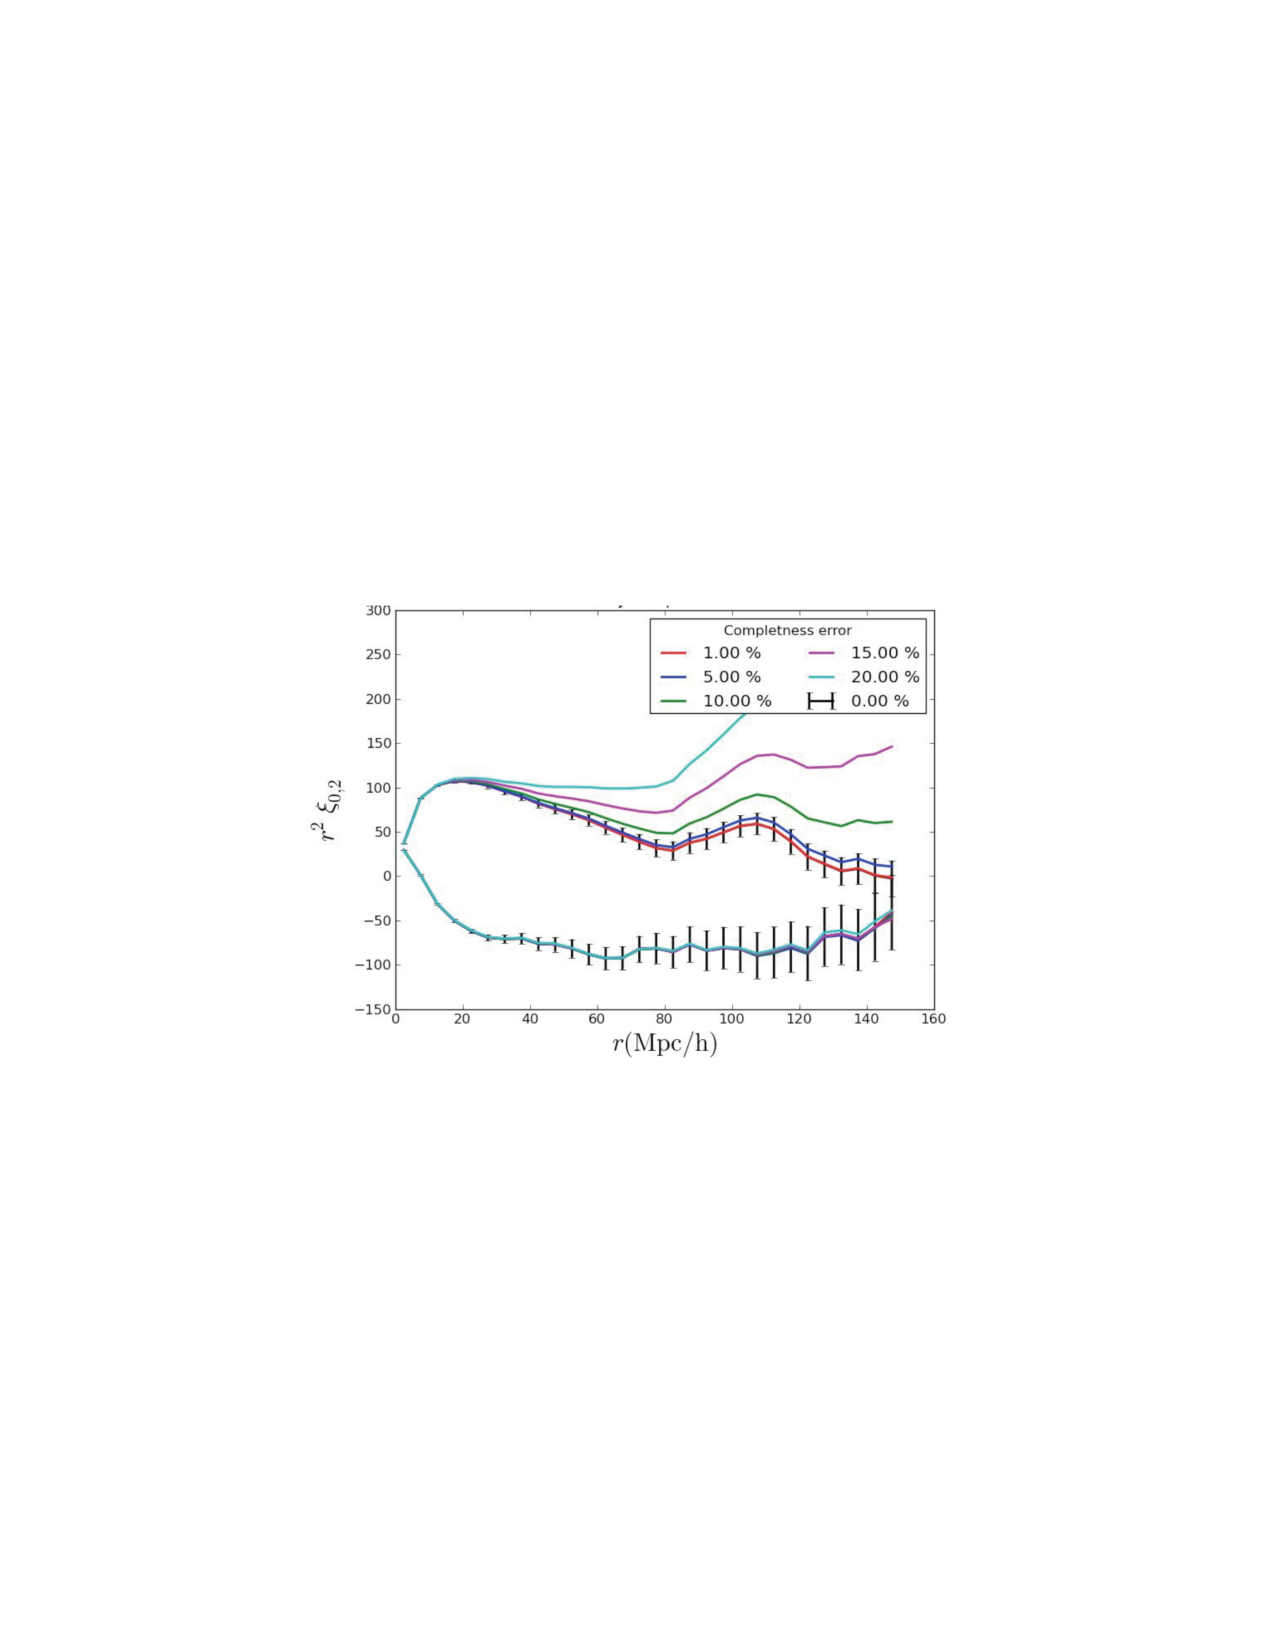
\includegraphics[width = 7in]{Plots/GRS_req_1July2016_v3_P6fig.pdf}
 \label{fig:selection_function}
 \vspace{-3.5in}
 \caption{\footnotesize{The monopole (upper curves) and quadrupole (lower curves) of a single mock
 survey and how they respond to various completeness errors in the scenario described in scenario.
 We can see from the level of two point correlation function, even a 5\% error on the completeness
 can change the monopole   and quadrupole significantly that we expect RSD to be affected, while
 BAO is not significantly affected, as this mostly changes the amplitude of the correlation function.
 }}
 %\begin{center}
 %\end{boxedminipage}
 \end{figure}

 (a)	The survey region is divided into two equal area along RA and one area
 has true completeness whereas the other one has $1-x$ completeness where x is a
 given completeness error (as shown in the legend of Figure \ref{fig:selection_function}).
 We show in Figure \ref{fig:selection_function} the resulting monopole and quadrupole with varying completeness error. This
 is an interesting limiting case as surveys can sometimes be affected by large
 scale systematics generated by either calibration of two parts of the sky, or
 due to large scale effects caused by the galactic foregrounds.

 (b)	The true survey completeness is multiplied with a gaussian function. The
 gaussian function has mean 0 and variance as the denoted completeness error. We
 then fold both positive and negative side of the Gaussian to the negative side
 and hence allow the completeness to be only smaller than its true value. We vary
 the scale at which we change the 3D selection function, starting with 1 degree
 to 4 degrees (4 deg is approximately the BAO scale at this redshift).
 %In particular, we will show the resulting monopole and quadrupole for 2 degrees and
 %4 degrees in Figure 3 and Figure 4 respectively. These are two interesting
 %limiting cases since they correspond to the extreme situation when the 3D
 %selection function are changed at scales most relevant to linear RSD modeling
 %and BAO analysis.

 From the preliminary analysis shown here, we expect that we will need to
 accurately model the 3D completeness function down to a few \% level.  At 5\%
 the effects can already be very detrimental to our large scale structure
 analyses using BAO and RSD. Scaling from these, we arrive at the requirement
 that artificial correlations due to inaccuracies in the 3D selection function
 are less than 10\% of the statistical error bars on scales smaller than 2
 degrees, and less than 20\% on larger angular scales.

 \subsubsection{Requirement on Cosmological Volume Simulations:}

 This is a new category of requirements for a space mission. These are not needed
 for mission success (data acquisition by the spacecraft), but for meeting the
 high level science requirements (level 1). We summarize these as follows:

 \begin{itemize}
 \item{(a) a few accurate mocks with galaxies included using semi-analytical
 galaxy formation model, to verify and validate WFIRST GRS pipeline; }
 \item{(b) $\sim 100$ mocks with high mass resolution of 109 solar masses, to inform theoretical
 modeling of the data; }
 \item{(c)$\sim 10,000$ mocks with low resolution, to derive
 the covariance matrices for the WFIRST data.}
 \end{itemize}

 To quantify the requirement on cosmological volume simulations, we consider only
 the case for galaxy clustering science (which includes BAO and RSD) for now for
 simplicity. For WFIRST, simulations are required for the following three
 objectives:  a. establishing the basic correctness of the pipeline; b.
 informing the theoretical modeling of small scale clustering as a function of
 tracer properties; c.	calculating the covariance matrix for each GRS probe and
 across many probes.

 In order to establish the basic correctness of the WFIRST pipelines and
 predictions, sophisticated synthetic mock galaxy catalogs are essential.
 These catalogs, which must realistically emulate WFIRST both in sky area and
 depth, are typically constructed by running large gravity-only simulations and
 then ``painting'' realistic galaxies on top.  Populating a simulation with
 galaxies can be done in several ways: (i) empirically, using statistics such as
 the ``halo occupation distribution'', (ii) by placing the normal, baryonic matter
 in the simulation ab initio and explicitly solving the hydro-dynamical
 equations, or (iii) by using a semi-analytical galaxy formation model (SAM),
 whereby the astrophysical processes and formation histories of galaxies are
 described using physically motivated, parameterized equations. The advantage of
 SAMs over alternative methods is their ability to meet the demands from next
 generation cosmological surveys for large (suites of) galaxy mock catalogues
 that are both accurate and can be constructed rapidly. In contrast, full
 hydro-dynamical simulations are far too slow and empirical methods are limited
 by the availability of existing high redshift observations, which are necessary
 for the calibration of these methods. SAMs also require some observations for
 calibration but, once tuned to fit observations at low redshift, they are able
 to make predictions out to high redshift without the need for further
 observational input. Furthermore, empirical methods are often limited in that
 they are calibrated in one or two photometric bands, whilst SAMs are designed to
 model the star formation history of a galaxy and so have the ability to make
 predictions for a wide variety of multi-wavelength data simultaneously. This
 feature of SAMs is vital to ensure that we can examine cross-correlations
 between the spectroscopically-selected dataset for galaxy clustering analysis
 and the photometrically-selected dataset for weak lensing analysis. Besides
 testing the pipeline and making (limited) cosmological forecasts, these galaxy
 mock catalogs would also be a valuable resource for science working groups
 focusing on legacy science (e.g. galaxy evolution, active galactic nuclei). Note
 that,  compared to the large number of approximate mock catalogs necessary for
 covariance estimation, only very few accurate galaxy mocks are required to
 verify and validate the WFIRST pipeline.


 To inform the theoretical modeling of clustering especially at non-linear
 scales as a function of the tracer properties would require a significant number
 of simulations that have relatively realistic modeling of the tracer properties
 at the relevant redshift.  For WFIRST, we can take the current number density of
 emission line galaxies (for H$\alpha$ galaxies only) from our baseline
 calculation and used the Tinker et al. 2008 halo mass function, along with the
 Giocoli et al. (2008) subhalo mass functions to compute the total number of
 halos and subhalos above some mass threshold and then match that to the baseline
 GRS number densities. This maps back to approximately 1012 solar masses from z=1
 to z=2. Assuming that we need to have at least 100 particles to resolve halos at
 1012 solar masses, and another factor of 10 particles to resolve properties of
 the halo progenitors, we will need dark matter particle mass resolution of
 approximately 109 solar masses. The extra factor of 10 is due to the galaxy
 formation model that depends on the properties of the progenitors which is an
 approximation that may change as we understand the galaxy properties better and
 as more observations of the tracers arrive. We expect to require of order 100
 simulations to reduce the shot noise of the correlation function in order to
 compare the theoretical modeling to the simulated correlation function. These
 realistic mock surveys may also require the modeling of non-standard
 cosmological  models, such as extensions to non-zero total neutrino masses, or
 modified gravity models.

 Finally, we will need to calculate the covariance matrices of the main probes of
 clustering, namely BAO and RSD, and the cross-covariances among these probes
 (or across different methods as in recent BOSS analyses). We can approach the
 calculation of the covariance matrices through multiple avenues. One can
 generate (in principle) a large number of approximate mock surveys using
 relatively fast approximate methods (eg. PTHalos, QPM, FastPM, etc), and apply
 the relevant survey properties onto these mock surveys. The small scale modeling
 of the clustering may not be 100\% accurate, but is likely to be adequate for
 the linear RSD modeling and BAO analyses where medium to large scales are most
 important. The number of approximate simulations required can be on the order of
 O(10,000) depending on the number of parameters we will be estimating using
 these covariance matrices, but the time requirement of these approximate mocks
 is relatively modest. One can also envision using more theoretical approaches
 (such as O'Connell et al. 2015, Padmanabhan et al. 2015), which only require a
 relatively modest number of realistic mock surveys which are required for (b).


 \subsection{Simulations}

 The KSU group has produced a suit of few thousand fast ``enhanced log-normal
 simulations'' for the WFIRST GRS expected samples. While these simulations do
 not correctly reproduce the small scale structure and higher order statistics of
 the field, they can be used for studying various large scale effects and
 implement light-cone effects. The simulations have so far been used to study the
 effect of splitting the WFIRST footprint into two non-contiguous areas. We plan
 to use this simulations in the future to study systematic effects in the
 measurements (e.g. window effect correction) and to validate the BAO/RSD
 proto-pipeline. These simulations are very well-suited for such tasks since
 their input two-pint signal is known exactly.

 \subsection{Cosmological Forecasting and Data Analysis Algorithms}

 The key dark energy constraints from the WFIRST GRS will result from the BAO and
 RSD measurements from the two-point statistics of the observed galaxy field.
 Similar measurements from the higher order statistics are weaker and currently
 are considered less robust. Cosmological constraints from higher order
 statistics scale very steeply with the number density and since WFIRST GRS will
 provide very dense galaxy samples they may significantly enhance the yield from
 the standard two-point BAO/RSD analysis. We also expect the methods of analysing
 higher order statistics to become more robust and standardized by the time of
 WFIRST launch. Because of this considerations it would be helpful to have a
 higher order statistics forecasting tool. We have developed software package to
 make forecasts on basic dark energy parameters from higher order statistics.
 The main assumptions are similar to the ones made in the standard
 power-spectrum forecasting tool used for baseline WFIRST predictions. We will
 work on integrating this software with the standard forecasting tool developed
 by our SIT. While the key design decisions will still be based on the
 two-point statistics forecasts, knowing how different choices will effect higher
 order analysis will be very informative.

 The KSU group has assembled a fast and lightweight set of tools for analysing
 the WFIRST GRS data. Currently this toolset starts from the redshift catalogue
 and the visibility cube and produces the measurements of power spectrum
 multipoles. The multipoles are then analyzed to extract the BAO and RSD signal
 from them. The BAO extraction algorithms replicate the analysis of the final
 BOSS DR12 sample. The RSD analysis is currently simplistic and uses the linear
 model. We will update this toolset by implementing more realistic RSD models.
 The toolset will eventually be linked to the redshift catalogue and visibility
 cube producing software. This software will provide the backbone of our BAO/RSD
 proto-pipeline and will be validated with high fidelity WFIRST simulations.




\Oli{SWITCHED HERE}

As discussed extensively in \S 2.2.4 of SDT15 (written by
members of our team), the defining goal of HLS spectroscopy is to derive
constraints on dark energy from a slitless spectroscopic (grism)
redshift survey of approximately 20 million emission line galaxies (ELG) in the redshift range $z=1-3$.
The galaxy redshift survey will enable high-precision measurements of the cosmic expansion history via BAO and structure growth via RSD.
Acoustic oscillations in the pre-recombination universe imprint a characteristic scale on matter clustering, which
can be measured in the transverse and line-of-sight directions to
determine the angular-diameter distance $D_A(z)$ and Hubble parameter $H(z)$, respectively \cite{Blake03,Seo03,CW12}.  Anisotropy of clustering
caused by galaxy peculiar velocities constrains (in linear perturbation
theory) the combination $\sigma_m(z) f_g(z)$, where $\sigma_m$ describes
the rms amplitude of matter fluctuations and $f_g(z) \equiv d\ln\sigma_m(z)/d\ln a$ is the fluctuation growth rate.
Thus the GRS on its own can address the key questions identified by
NWNH: whether cosmic acceleration is caused by modified gravity
or by dark energy, and whether (in the latter case) the dark energy
density evolves in time \cite{Guzzo08,Wang08}.  These tests become more powerful in
combination with weak lensing and cluster measurements from HLS Imaging
and high-precision relative distance measurements from the Supernova
Survey \cite{dePutter:2013xda,dePutter:2013nha}. The broadband shape of the galaxy power spectrum and higher order
measures of galaxy clustering provide additional diagnostics of
dark energy, neutrino masses, and inflation, and insights on the physics of galaxy formation.
%There are two largely distinct sources of systematics in the galaxy clustering program, associated with
%the uniformity of the GRS and with astrophysical modeling uncertainties.
%We discuss these in \S\ref{sec:grs_requirements} and~\S\ref{sec:grs_forecasting}, respectively, and we briefly
%discuss mitigation strategies in \S\ref{sec:grs_mitigation}.
While all aspects of our GRS investigation are interconnected, we
organize it in a structure similar to that of \S
\ref{sec:wl_gal-clusters} for clarity: requirements, simulations, and prototype pipelines in \S \ref{sec:grs_requirements},
cosmological forecasting, modeling, and cosmological simulations in \S
\ref{sec:cmethods}, and systematics testing and mitigation in \S \ref{sec:gal_syst}.


\subsection{Requirements}
\label{sec:grs_requirements}
\Auth{Yun, Lado}

The most important task of the SIT in guiding
development of the WFIRST HLS spectroscopy is to set and validate the
requirements of the instrument, the data reduction software, and the survey.
The GRS Lead Co-I Wang will work closely with PI Dor\'e and Co-Is
Hirata and Teplitz on setting requirements for the GRS. To make fully
informed decisions, the team requires high fidelity simulations of
both
instrument performance and the observable sky that the instrument will
measure.  The team must also ensure that the analysis of these data by
the reduction pipeline will be of sufficient quality to enable
measurement with the high precision needed for cosmology.
These simulation and pipeline activities will require the team to
coordinate with the WSC.  Several members of our team (Wang, Teplitz,
Capak, Helou) are located at the Infrared Processing and Analysis
Center (IPAC), and work closely with the WSC.
%\Oli{Mention George too if he stays in}%The WSC task plans are still under discussion, but will
%most likely include development of a pixel-level simulator for imaging
%and spectroscopy.  They will (certainly) include the construction of a
%production-quality analysis pipeline to remove detector effects and
%(probably) extract and measure emission-line spectra.
To the extent practical, we will draw on tools created by the WSC and
design our own software and simulations to be useful to them.
We note that our work primarily demands the ability to quickly and flexibly
simulate different configurations and analyze the results with different
algorithms, while the WSC has the task of developing tools for the
community and production
ready pipelines that integrate with the full WFIRST data system.

\subs{Deriving requirements.} As with WL (\S\ref{sec:wl_requirements}), we will focus first on GRS
requirements that may drive hardware choices, i.e., those that may be
demanding in terms of grism design, detector properties, stability and repeatability of pointing, or dedicated calibration hardware.
We will include a prioritized list of effects to
incorporate in grism simulations.  Over time, we will use our
increasingly realistic network of simulations to evaluate the impact
of requirements and possible trades from the pixel level through
to cosmological inferences. The starting points for this
process are the WFIRST ETC and survey planning software
and the \CoLi\ forecasting tool.

The maximum achievable statistical power of the GRS is determined
mainly by the telescope aperture, throughput, detector area and pixel
size, and allotted observing time.  However, the statistical power and
uniformity of the GRS are further affected by numerous aspects of
instrument performance and survey design, e.g., spectral resolution,
detector read noise and persistence, dither and roll angle pattern,
image quality, complexity of non-1$^{\rm st}$ order features,
spatially varying thermal background due to the warm telescope,
scattered light from bright stars, repeatability of the grism
positioning, and accuracy of calibration of the wavelength-dependent
PSF and distortion map.

Non-uniformity of the survey, which is inevitable to some degree, can
be corrected in clustering measurements by weighting galaxies to
account for incompleteness.  However, large corrections typically come
at a cost in statistical power, and imperfect knowledge of the
non-uniformity leads to systematic errors in the inferred clustering.
The other important source of observational systematics is
contamination of the redshift catalog by artifacts or objects with
incorrectly determined redshifts, and loss of objects from the catalog
because of catastrophic redshift errors or uncertainties in the flux
calibration.  We will define requirements such that (a) the
statistical power of the GRS is close to the maximum allowed by the
telescope aperture and detector area and (b) the impact of uncorrected
observational systematics is small compared to the statistical
errors. The expected precision of the galaxy power spectrum provides a
useful guide to the statistical power of the GRS, but the full
question of cosmological constraining power depends on the
astrophysical modeling techniques used to interpret the measured
clustering, as discussed in \S\ref{sec:cmethods} below.  By the end of our
investigation we will have a complete set of tools to evaluate the
impact of hardware or strategy trades, changes in requirements, or
changes in astrophysical inputs on the expected cosmological return
from the GRS.

\subs{Simulations.} Our development of requirements and a prototype spectroscopic
pipeline will rely critically on realistic simulations of the
pixel-level grism images.  We will work closely with the WSC on
developing these simulations for a variety of cases, ranging from
simple widely separated sources to realistically clustered galaxy
populations drawn from the cosmological simulations described in
\S\ref{sec:cmethods}.  Our team has extensive experience in producing
such simulations for the Hubble Space Telescope (HST) and Euclid.  Co-I Tepliz is one of the leaders
of the HST Wide-Field Camera 3 (WFC3) IR Spectroscopic Parallel survey (WISPs), for which
pixel simulations are vital in assessing completeness and other
parameters \cite{Colbert13}; Co-I Wang (with Teplitz and Capak) is
developing simulation techniques for the Euclid grism survey.
Co-I Teplitz will lead our grism simulations for WFIRST.
A critical astrophysical input for these simulations is the
redshift-dependent luminosity function of H$\alpha$ and [OIII]
emitters, which is currently uncertain at levels that have an
important impact on WFIRST strategy and performance forecasts.  Co-Is
Teplitz and Wang are part of an HST archival study to reprocess
existing data from multiple HST projects to mitigate systematic
uncertainties of the H$\alpha$ luminosity function (LF) measurement.  Through WISPs, Teplitz
is also working to obtain significantly more HST data to improve the
H$\alpha$ LF measurement.  In addition, realistic galaxy templates are
vital to the forecasting of grism measurements, and we are working to
improve both line diagnostics and prediction of line vs. continuum
properties.

\subs{Prototype pipeline.} We will build a prototype spectroscopic pipeline for the analysis of
slitless spectroscopic data to produce a redshift catalog.  This is a
complex, multi-step process.  Co-I Teplitz has extensive experience
with HST slitless spectroscopy using the WFC3, HST Near Infrared Camera and
Multi-Object Spectrometer (NICMOS), and HST Space Telescope Imaging
Spectrograph (STIS) instruments \cite{Atek10,Shim09,Teplitz03}; he
will lead our work on prototype pipelines for the GRS. We will take the basic steps
implemented for WFC3 processing as the starting point for a prototype
WFIRST pipeline. This pipeline must clean the grism images of contamination
from detector artifacts and cosmic rays, register and combine images
from separate dithers and roll angles, match objects in the dispersed
and direct imaging exposures, extract wavelength- and flux-calibrated
2D spectra, infer redshifts based on detected emission lines, and
measure emission-line fluxes and other spectroscopic characteristics.
The resulting catalogs are the input for the clustering analyses
discussed further in \S\ref{sec:cmethods}.

\subs{Analysis challenges.} Slitless spectroscopic analysis presents several important challenges.
First, the pipeline must mitigate the confusion caused by overlapping
spectra.  The standard solution (used by the HST data pipeline) is to
subtract a model of neighboring objects from each source as it is
extracted.  We will investigate the use of HST-like algorithms for
WFIRST, as well as more sophisticated solutions that could produce
better results, such as fitting the full pixel set for regions of the
frame.  Model dependent solutions, with iterative fitting, are
potentially promising, but biases would have to be carefully
understood.  While the HLS obtains exposures at multiple roll angles,
these may be greatly separated in time.  This could introduce new
problems for variable sources, or in fields with foreground moving
objects.  We will also develop methods to automate quality assessment
and flagging of extracted spectra, as the sheer volume of WFIRST GRS
will make human review of spectra (standard practice in current grism
surveys) impossible.

A second major challenge is the need to mitigate catastrophic redshift
errors.  Such failures arise from the misidentification of redshifts
(e.g., confusing [OIII] for H$\alpha$\ in low signal to noise (S/N) spectra) or
false-positive line detections caused by noise peaks or unflagged
cosmic rays.  Redshift fidelity can be greatly improved by using the
photometric redshift estimates derived from the multi-band photometry as a prior
in the redshift determination.  Co-I Capak is spearheading
multidimensional analysis of galaxy color information for WFIRST
photometric redshifts, and that work will be folded into the
spectroscopic pipeline.
% (\Oli{PETER SHOULD DOUBLE CHECK THE WORDING HERE}).

\subs{Completeness maps.} Nearly as important as the redshift catalogs themselves is the production of
completeness maps that characterize the spatially varying depth of the survey,
the level of contamination, and regions that should be masked because the
catalog is unreliable.  These completeness maps are used to weight galaxies in
clustering analysis and/or to create random catalogs such that the local number
density of points is proportional to the likelihood of successfully measuring a
redshift of a galaxy if it were at that point.  Co-I Samushia is
leading a similar effort in DESI and has previously worked on quantifying and removing
systematic effects associated with inaccuracies in random catalogues
\cite{Samushia2012}.
Co-I Ho has also led the effort in creating the SDSS-BOSS LSS catalog and randoms \cite{Reid2015} and led the effort in removing observational effects in BOSS LSS catalog \cite{Ross2011}.
Co-I Samushia will lead our work to develop tools for creating these completeness maps
by a full forward-modeling method, where artificial sources are assigned random
angular positions and redshifts, added to grism images, and pushed through the
data pipeline.  Compared to existing large redshift surveys (from ground-based
fiber spectroscopy), the WFIRST completeness map will have much more complex
small scale structure because of the varying numbers of exposures at individual
points on the sky and sensitivity variations across the focal plane.  Because of
source confusion and sky background effects, the completeness and contamination
will be a function of the local galaxy surface density.  We will develop
strategies and tools for recording these large and complex completeness maps in
formats that can be efficiently used to create random catalogs and weight
galaxies for clustering analyses.  By the end of the investigation period, we
will be able to create full pixel-level simulations from an input cosmological
simulation (see \S\ref{sec:cmethods}), run them through our proto-type pipeline to create a
redshift catalog and completeness map, and analyze the resulting artificial data
set with our clustering analysis tools to compare to the idealized case that has
the complete galaxy catalog of the cosmological simulation.

\subs{Calibration strategies.}
We will define the absolute and relative calibration requirements for the GRS, such as the angular scale and temporal stability.
We will develop methods for calibrating the relative and absolute flux measurements along with wavelength calibration and redshift accuracy and completeness.
For flux and wavelength calibration we will set requirements on the ground testing, in flight calibration sources, and calibration observations based on experience
with other missions including Spitzer, HST, and Euclid.  Furthermore, we will investigate self calibration strategies based on optimizing dither patterns and exposure
times for the science observations and the use of touch-stone fields that both calibrate and provide long-term trending of the data.  Both the primary and
self calibration procedures will be tested with simulations specified by this SIT and conducted by the WSC.  Finally, we will use the large spectroscopic surveys
necessary for the weak lensing photo-$z$ calibration to verify the calibration by directly testing the redshift accuracy and completeness estimates from the simulations.
Co-Is Capak and
Padmanabhan, both with extensive experience from similar work for
Euclid and BOSS, will lead our calibration work.

\subsection{Simulations}
\label{sec:grs_simulations}
\Auth{Shirley, Elena, Andrew, Alina, Alex, Yun}


%===
% \subsection{Requirements, Simulations, and Proto-type Pipelines}


% The most important task of the SIT in guiding
% development of the WFIRST HLS spectroscopy is to set and validate the
% requirements of the instrument, the data reduction software, and the survey. To make fully informed
% decisions, the team requires high fidelity simulations of both
% instrument performance and the observable sky that the instrument will
% measure.  The team must also assure that the analysis of these data by
% the reduction pipeline will be of sufficient quality to enable
% measurement with the high precision needed for cosmology.
% These simulation and pipeline activities will require the team to work
% closely with the WFIRST Science Centers (WSC).  Several members of our team
% (Wang, Teplitz, Capak) are located at IPAC, and they work closely with
% the WSC. %The WSC task plans are still under discussion, but will
% %most likely include developmet of a pixel-level simulator for imaging
% %and spectroscopy.  They will (certainly) include the construction of a
% %production-quality analysis pipeline to remove detector effects and
% %(probably) extract and measure emission-line spectra.
% To the extent practical, we will draw on tools created by the WSC and
% design our own software and simulations to be useful to the WSC.
% We note that our work primarily demands the ability to quickly and flexibly
% simulate different configurations and analyze the results with different
% algorithms, while the WSC has the task of developing production
% ready pipelines that integrate with the full WFIRST data system.

% As with WL (\S\ref{sec:wl_requirements}), we will focus first on GRS requirements that may drive hardware choices, i.e., those that may
% be demanding in terms of grism design, detector properties, stability
% and repeatability of pointing, or dedicated calibration hardware.
% Our initial assay will include a prioritized list of effects to incorporate in grism simulations.  Over time, we will use our
% increasingly realistic network of simulations to evaluate the
% impact of all requirements and possible trades from the pixel level through to cosmological inferences.  The starting points for this
% investigation are the WFIRST ETC and survey planning software (both written by Co-I Hirata) and the CosmoLike forecasting tool
% described in \S\ref{sec:wl_requirements}.

% The maximum achievable statistical power of the GRS is determined
% mainly by the telescope aperture, throughput, detector area and pixel size,
% and allotted observing time.  However, the statistical power and uniformity of the GRS
% are further affected by numerous aspects of instrument performance and survey design:
% spectral resolution, detector read noise and persistence, dither and roll angle pattern,
% blurring due to diffraction by the glass elements of the grism, spatially varying thermal
% background due to the warm telescope, scattering due to bright
% stars, repeatability of the grism positioning, and accuracy of
% calibration of the wavelength-dependent PSF and distortion map.

% Non-uniformity of the survey, which is inevitable to some degree,
% can be corrected in clustering measurements by weighting galaxies
% to account for incompleteness.  However, large corrections typically come
% at a cost in statistical power, and imperfect knowledge of the
% non-uniformity leads to systematic errors in the inferred clustering.
% The other important source of observational systematics is
% contamination of the redshift catalog by artifacts or objects with incorrectly
% determined redshifts, and loss of objects from the catalog
% because of catastrophic redshift errors.
% We will define requirements such that (a) the statistical power of
% the GRS is close to the maximum allowed by the telescope aperture
% and detector area and (b) the impact of uncorrected observational
% systematics is small compared to the statistical errors. The expected precision of
% the galaxy power spectrum provides a useful guide to the statistical power of the GRS, but the full
% question of cosmological constraining power depends on the
% astrophysical modeling techniques used to interpret the measured
% clustering, as discussed in \S 5.2 below.
% By the end of our investigation we will have a complete set of
% tools to evaluate the impact of hardware or strategy trades,
% changes in requirements, or changes in astrophysical inputs
% on the expected cosmological return from the GRS.

% Our development of requirements and a proto-type spectroscopic pipeline
% will rely critically on realistic simulations of the pixel-level
% grism images.  We will work closely with the WSC on developing
% these simulations for a variety of cases, ranging from simple
% widely separated sources to realistically clustered galaxy populations
% drawn from the cosmological simulations described in \S 5.2.
% {\bf Can we say more here?  Do we have any experience producing
% grism simulations for HST analysis?}
% A critical astrophysical input for these simulations
% is the redshift-dependent luminosity function of H$\alpha$ and [OIII]
% emitters, which is currently uncertain at levels that have
% an important impact on WFIRST strategy and performance forecasts.
% Co-I's Teplitz and Wang are part of an HST archival study to reprocess existing
% data from multiple HST projects to mitigate systematics uncertainties of the
% H$\alpha$ LF measurement.  Teplitz is also a key member of the WISP team,
% which aims to obtain significantly more HST data to improve the H$\alpha$ LF measurement.

% We will build a prototype spectroscopic pipeline for the
% analysis of slitless spectroscopic data to produce a redshift catalog.
% This is a complex, multi-step process.
% Co-I Teplitz has extensive experience with the HST grism data
% pipeline (e.g., \cite{REFS}), and we will take the algorithms
% implemented in this pipeline as the starting point for a
% proto-type WFIRST pipeline. This pipeline must clean the grism images for contamination from
% detector artifacts and cosmic rays, register and combine images from
% separate dithers and roll angles, extract wavelength- and flux-calibrated
% 2D spectra, match these spectra
% to individual objects from the photometric imaging data,
% infer redshifts based on detected emission lines, and measure
% emission-line fluxes and other spectroscopic characteristics.
% The resulting catalogs are the input for the clustering analyses
% discussed further in \S 5.2.

% The biggest challenge for slitless spectroscopic analysis is
% eliminating confusion from overlapping spectra.
% The standard solution (used by the HST data pipeline) is to subtract a
% model of neighboring objects from each source as it is extracted.
% We will investigate the use of HST-like algorithms for WFIRST,
% as well as more sophisticated solutions that could produce better results,
% such as fitting the full pixel set for regions of the frame.
% Model dependent solutions, with iterative fitting, are potentially
% promising, but biases would have to be carefully understood.
% While the HLS obtains exposures at multiple roll angles, these may
% be greatly separated in time.  This could introduce new problems for variable sources, or in fields with foreground moving objects.
% We will also develop methods to automate quality assessment
% and flagging of extracted spectra, as the sheer volume of WFIRST GRS will make human review of spectra
% (standard practice in current grism surveys) impossible.

% Another challenge is the misidentification of noise peaks as emission lines, which leads to
% catastrophic redshift errors. This can be mitigated by using the photometric redshift derived from
% the multi-band photometry as a prior in the redshift determination.

% Nearly as important as the redshift catalogs themselves is the
% production of completeness maps that characterize the spatially
% varying depth of the survey, the level of contamination, and
% regions that should be masked because the catalog is unreliable.
% These completeness maps are used to weight galaxies in clustering
% analysis and/or to create random catalogs such that the local number
% density of points is proportional to the likelihood of successfully measuring a redshift of a galaxy if it were at
% that point.  We will develop tools for creating these completeness
% maps by a full forward-modeling method, where artificial sources
% are assigned random angular positions and redshifts, added to
% grism images, and pushed through the data pipeline.
% Compared to existing large redshift surveys (from ground-based
% fiber spectroscopy), the WFIRST completeness map will have much
% more complex small scale structure because of the varying numbers
% of exposures at individual points on the sky and sensitivity
% variations across the focal plane.
% Because of source confusion and sky background effects,
% the completeness and contamination will be a function of
% the local galaxy surface density.
% We will develop strategies and tools for recording these large and
% complex completeness maps in formats that can be efficiently
% used to create random catalogs and weight galaxies for clustering
% analyses.  By the end of the investigation period, we will be able
% to create full pixel-level simulations from an input cosmological
% simulation (see \S 5.2), run them through
% our proto-type pipeline to create a redshift catalog and completeness
% map, and analyze the resulting artificial data set with our
% clustering analysis tools to compare to the idealized case
% that has the complete galaxy catalog of the cosmological simulation.


\subsection{Cosmological Forecasting, Modeling, and Simulations (D2, D8, D9)}
\label{sec:cmethods}
%================================================
%\Auth{Yun, Katrin, Nikhil, Rachel B, Alina, Shirley, Olivier}

\subs{Forecasting.} Our initial forecasts for the cosmological constraints from
the WFIRST GRS will adopt the model-independent approach (incorporating
both BAO and RSD) that Co-I Wang has developed \cite{Wang2013} and
used for the WFIRST SDT reports and similar forecasts for Euclid \cite{WangEuclid2010}.
This approach offers a fast way to forecast how uncertainties in
$H(z)$, $D_A(z)$, growth rates, and other cosmological parameters
change in response to changes of the survey strategy, instrument
performance, or astrophysical inputs such as the H$\alpha$ luminosity
function.  Early in this investigation, we will incorporate a full description
of redshift-space galaxy clustering into \CoLi, using a halo
occupation density (HOD) framework similar to that already implemented for
angular galaxy clustering \cite{Krause2013}.  In the medium term, we will also
incorporate effects of clustering measurement and theoretical
modeling systematics via nuisance parameters, analogous to our
existing treatments of observational and theoretical systematics
in weak lensing analysis.  The expected level of these systematics
will be informed by the studies described in \S\ref{sec:grs_requirements}
and below.  As with the imaging survey, this comprehensive forecasting
framework will enable us to connect low-level technical requirements
to our top-level science goals.

\subs{GRS modeling.} The development of the methodology for the
interpretation of GRS data is centered on the mitigation of the
astrophysical systematic effects  for galaxy clustering measurements:
nonlinear effects, RSD (growth rate signal on large scales and
contamination on small and intermediate scales),  and galaxy bias (the
difference between galaxy and matter distributions).
Co-I Padmanabhan is a leading expert in BAO/RSD data analysis \cite{Padmanabhan2007,Padmanabhan2008,Padmanabhan2009,Padmanabhan2012,Xu2012}; he will lead our
work in GRS modeling/interpretation methods, with participation from the PI and Co-Is
Bean, Ho, Samushia, Spergel, Wang, and Weinberg \cite{CW12,Ho2012,Anderson2014,Wang2014,Osumi2015,Alam2015a,Alam2015b,Cuesta2015}.

BAO measurement is now a mature field, but WFIRST probes new regimes
of precision and redshift using different instrumental choices
and different classes of galaxy tracers from previous surveys.
Effects of non-linear clustering and galaxy bias are expected to
influence BAO measurements at the $\sim 0.5\%$ level \cite{Padmanabhan2009}, which is
significant compared to WFIRST statistical errors.
Reconstruction methods \cite{Eisenstein2007,Padmanabhan2012,Vargas2015},
which attempt to reverse the
nonlinear evolution of the BAO feature, appear to remove
most of this effect while simultaneously improving the precision
of BAO measurements.  Current observational studies use very simple
reconstruction algorithms.  We will explore more sophisticated
reconstruction methods, building on low redshift work \cite{Carrick15}, and test their performance on simulations
of WFIRST galaxy redshift catalogs, including realistic treatments of
survey geometry, redshift evolution, source space density, and
variable completeness.  Building on current work by Co-Is
\cite{Padmanabhan2012,Vargas2015,Osumi2015,Zhu2015},
we will also investigate improved clustering estimators that can sharpen the precision and improve the robustness
of BAO measurements.

In sharp contrast to BAO measurements, cosmological inference from
RSD measurements is already limited mainly by uncertainties in
theoretical modeling, with application of different models to the
same underlying data yielding differences at the $\sim 10\%$ level.
%{\bf SH: Not sure it is 5\% level, I think BOSS results differ by
%nearly 10\% level with the mock challenge} .
Furthermore, the statistical signal-to-noise ratio of RSD measurements
increases rapidly with decreasing scale, so there are potentially
large gains from modeling that extends into the fully non-linear regime.
We will pursue a variety of approaches to improving and testing
RSD models, including the
%{\bf not calling this brute force ? } ``brute force''
efficient method of computing predictions
numerically by populating the halos of N-body simulations with galaxies.
Co-I Spergel has expertise in combining imaging and spectroscopic
data to predict the relationship between galaxies and halos \cite{Hikage2012}.
One can think of this method as producing ``emulators'' \cite{Heitmann2014}
that predict galaxy clustering statistics as a function
of cosmological parameters and parameters that describe the relation
between galaxies and dark matter halos.
The approach shows promise (e.g., \cite{Reid2014}),
but it relies on parameterized models for populating halos,
and the accuracy of these needs to be tested against galaxy catalogs
constructed in ways that do not share the same assumptions
(e.g., by semi-analytic models or abundance-age matching).
We will use similar techniques to investigate the impact of
non-linear evolution and bias on the broadband galaxy power
spectrum, and thus improve our ability to extract cosmological
information from this measurement.

Galaxy bias is likely scale-dependent; its testing will require realistic ELG mocks, and its mitigation will require
the successful measurement of the higher-order statistics of galaxy clustering, which in turn requires a
sufficiently high galaxy number density for the GRS.
An essential difference between the WFIRST and Euclid spectroscopic
surveys is that due to the much smaller pixel scale (0.11$^{\prime\prime}$ for WFIRST
versus 0.3$^{\prime\prime}$ for Euclid) and larger telescope aperture, WFIRST
is capable of carrying out a significantly deeper GRS, which can result in
%, at least as currently planned, is the
a much higher space density of the WFIRST sample over most
of its redshift range.
This high sampling density represents a significant science opportunity
for WFIRST;
in particular it will boost the significance of higher-order correlations.
Building on previous work by members of our team \cite{Takada08,Schaan14,Dore14,Chen15},
%(Takada et al. 2008; Schaan, Takada \& Spergel 2014; Chen, Ho et al. 2015),
we will investigate techniques that use the galaxy
bispectrum and other higher-order statistics to sharpen cosmological
constraints, by directly probing the matter density and velocity fields
and by improving knowledge of ``nuisance parameters'' that describe
galaxy bias.  We will examine ways that RSD measurement precision
can be improved by cross-correlating multiple tracer populations
with different clustering bias to suppress cosmic
variance \cite{mcDonald2009,Bernstein2011,dePutter:2014lna}, weighting galaxies by mass
to suppress shot noise \cite{Seljak2009}, and building group catalogs
to collapse fingers-of-God \cite{Reid2010}.
We will investigate potential gains from cross-correlating the
WFIRST galaxy redshift catalogs with H$\,${\sc i} 21 cm ``intensity mapping''
measurements, or with CMB measurements, or (at $z>2$) the Ly$\alpha$ forest.
In all of these studies, we will pay particular attention to
the influence of the sampling density, as this directly informs
the trade between depth and area in the GRS (see \S\ref{sec:sur_opt}).

\subs{Cosmological simulations.} The cosmological simulations described in \S\ref{sec:wl_methodology}
will also be useful for the methodology development outlined above.
However, the optimal simulations for BAO and RSD studies will typically
be larger volume and lower resolution than those for weak lensing:
large volumes are needed for good statistics and to eliminate finite
box effects, but we do not need to model the small scale matter
distribution or baryonic effects (which are encoded in the
models used to populate halos with galaxies).  Furthermore,
simulations tuned to the WFIRST GRS need only be evolved to $z=1$.
Co-I Ho will lead our cosmological simulations for the GRS, with participation from
team members Benson, Heitmann, Kiessling, Wang, and postdocs.

We will leverage the participation of several of our team members in
Euclid and DESI to produce large simulated ELG catalogs,
building on work we have already begun for these projects.
To model emission-line selection, we will use both semi-analytic galaxy
formation models (SAM) and HOD models that are tuned to produce
observed number densities and clustering.
%The current Euclid ELG mocks are made using SAM, but are limited in emission line modeling
%and simulation volume.
We expect to be able to provide ELG mocks for WFIRST similar to those used
by Euclid on a short time scale.
We will incorporate these into the early pixel-level
simulations described in \S\ref{sec:grs_requirements},
which will in turn be used to assess impacts of incompleteness,
contamination, and redshift errors on the galaxy distribution.

We will base our first cosmological volume ELG catalogs on two very large simulations
that are already available to us through collaborator Heitmann:
the Outer Rim simulation, covering
a volume of $4.225\,{\rm Gpc}^3$ with a particle mass of
$\sim 2\times 10^9 M_\odot$,
and the Q Continuum simulation, covering a volume of $1.3\,{\rm Gpc}^3$
with particle mass of $\sim 10^8 M_\odot$.
The Outer Rim simulation was used to create the simulated ELG
catalog for DESI.
We will combine the halo populations from these simulations with the
\textsc{Galacticus} semi-analytical galaxy formation model \cite{Benson2010,Benson2012} to create clustered ELG catalogs,
some in fixed-redshift cubes for methodology tests and some in light cones
with realistic survey geometry and redshift evolution.
Our most ambitious simulation efforts, later in the investigation
period, will take full light-cone ELG catalogs, create pixel-level
simulations that span the entire HLS area, and analyze these simulations
with the proto-type pipeline to produce ``observed'' galaxy catalogs.
We can then apply the full clustering measurement machinery
(including corrections for varying completeness) to these catalogs
and apply our cosmological inference tools
to understand the impact of observational systematics on
cosmology from the WFIRST GRS.
As with the weak lensing investigation, we will investigate computational
requirements beyond FY20 and techniques to reduce them. We will also make our
simulations publicly available so that others can develop and
test their own methods, with some of them released in the form of blind
data challenges.


\subs{H{$\rm \alpha$} emitter number density forecasts.} In work led
by Merson, Wang, Benson, Kiessling and Rhodes the open source
semi-analytical galaxy formation model, \textsc{Galacticus}
\cite{Benson2010,Benson2012}, was used to predict the H${\rm
  \alpha}$-emitter number counts and redshift distributions for the
WFIRST GRS.

A four square degree lightcone catalogue was constructed by processing
the dark matter merger trees of the Millennium Simulation
\cite{Springel05} with the \textsc{Galacticus} model. Emission lines
are modelled in \textsc{Galacticus} by interpolating over a library of
emission line luminosities obtained from the \textsc{Cloudy}
\cite{Ferland13} code and stored as a function of hydrogen (HI),
helium (HeI) and and oxygen (OII) ionising luminosities, as well as
the hydrogen gas density and metallicity of the interstellar medium
(ISM). The emission line luminosities are then processed to
incorporate attenuation due to interstellar dust, which can be
modelled using several different methods. Merson and collaborators
consider three dust methods from Ferrara \textit{et al.} (1999)
\cite{Ferrara99}, Charlot \& Fall (2000) \cite{Charlot00} and Calzetti
\textit{et al.} (2000) \cite{Calzetti00}. However, it is worth noting that any
user-specified dust method can be used in conjunction with
\textsc{Galacticus}.

\begin{figure}
  \centering
  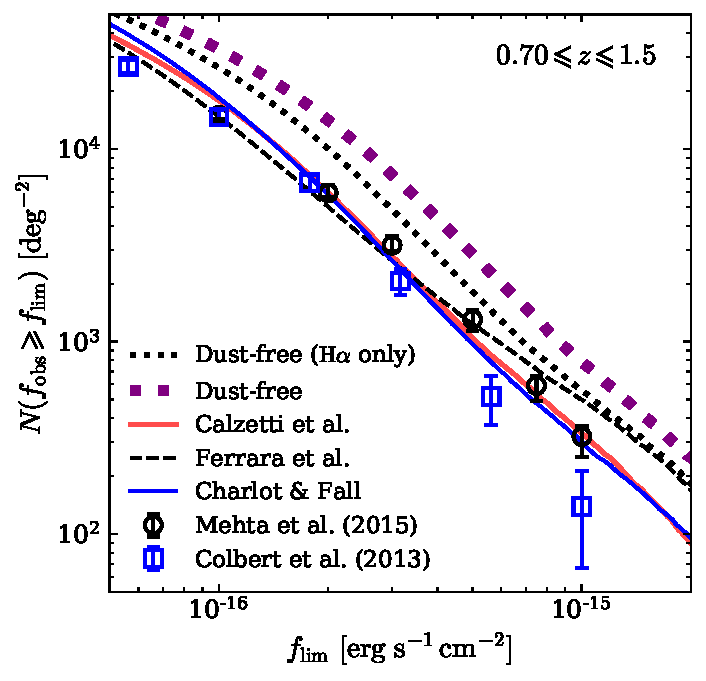
\includegraphics[width=3.5in]{Plots/merson17LightconeHalphaCumulativeCounts.pdf}
  \caption{Predictions for the cumulative H${\rm \alpha}$ flux counts
    for the redshift range $0.7<z<1.5$ from a \textsc{Galacticus}
    lightcone mock catalogue. The various lines show the predictions
    for the pure H${\rm \alpha}$ fluxes and the H${\rm \alpha}$ fluxes
    when blended with NII (H${\rm \alpha}+{\rm NII}$), assuming either
    no dust attenuation or attenuation using one of three methods:
    Ferrara \textit{et al.} (1999) \protect\cite{Ferrara99}, Charlot
    \& Fall (2000) \protect\cite{Charlot00} or Calzetti \textit{et
      al.} (2000) \protect\cite{Calzetti00}. To be consistent with
    the observed counts from WISP \protect\cite{Colbert13,Mehta2015},
    which are shown by the data points, contamination from NII is
    assumed to contribute 29 per cent to the galaxy luminosity.}
  \label{fig:halpha_flux_counts}
\end{figure}


First, the \textsc{Galacticus} predictions for the cumulative counts
of H${\rm \alpha}$-emitting galaxies over the redshift range
$0.7\leqslant z\leqslant 1.5$ obtained with each dust method are
compared with the latest WISP counts from Mehta \textit{et al.} (2015)
\cite{Mehta2015}. The H${\rm \alpha}$ luminosities from
\textsc{Galacticus} are corrected to introduce contamination due to
NII by assuming that NII contributes 29\% to the observed emission
line luminosity. A fixed NII contamination was chosen to be consistent
with the WISP analyses of Colbert \textit{et al.} (2013)
\cite{Colbert13} and Mehta \textit{et al.} \cite{Mehta2015}. Adjusting
the strength of the attenuation in two of these dust models, the
Charlot \& Fall \cite{Charlot00} method and the Calzetti \textit{et
  al.}  \cite{Calzetti00} dust law, leads to \textsc{Galacticus}
yielding cumulative H${\rm \alpha}$ flux counts that are consistent
with the observed counts of Mehta \textit{et al.}  \cite{Mehta2015}
down to a flux limit of $1\times 10^{-16}{\rm erg}\,{\rm s}^{-1}{\rm
  cm}^{-2}$ (see Figure~\ref{fig:halpha_flux_counts}). Adopting the
Ferrara \textit{et al.} \cite{Ferrara99} dust method yields counts
that agree with the observations for flux limits fainter than
approximately $5\times 10^{-16}{\rm erg}\,{\rm s}^{-1}{\rm cm}^{-2}$,
but predict an excess in the number counts for the brightest
fluxes. Overall, this work shows that down to the expected flux limits
of the WFIRST mission, the \textsc{Galacticus} model is able to
predict number densities that are consistent with existing
observations from the WISP survey. Although the lightcone used in this
analysis has a small area on the sky, it is expected that cosmic
variance has little effect on the predicted number counts. Since the
lightcone analysis is time-consuming and expensive in computing
resources, the lightcone used in this study was limited in size to 4
sq deg, in order to provide timely input to WFIRST. However,
significantly larger lightcones will be built in the future.

As a consistency check, the authors show that \textsc{Galacticus}, in
combination with the revised dust attenuation strengths, is consistent
with the observational estimates for the distribution of optical
depths (at the observer-frame H${\rm \alpha}$ wavelength) as well as
the H${\rm \alpha}$ line luminosity function, though at $z> 1.5$ the
luminosity function from \textsc{Galacticus} progressively a worse fit
to the observations. This could suggest that the dust methods may be
lacking some redshift evolution or dependence on other galaxy
properties, or that the \textsc{Galacticus} emission line luminosities
are the incorrect strength. Investigating these possibilities requires
rigorous calibration of the \textsc{Galacticus} model, which will be
carried out in future work.


\begin{table*}
\centering
\caption{\textsc{Galacticus} predictions for the cumulative number of
  H${\rm \alpha}$-emitting galaxies for the WFIRST GRS, assuming a
  redshift range of $0.5\leqslant z\leqslant 2$. The upper half of the
  table shows the counts for NII contaminated fluxes, whilst the lower
  half of the table shows the counts when NII contamination is
  removed. Predicted counts are reported for three dust methods:
  Calzetti \textit{et al.} (2000) \protect\cite{Calzetti00}, Charlot
  \& Fall (2000) \protect\cite{Charlot00} and Ferrara \textit{et al.}
  (1999) \protect\cite{Ferrara99}. For the Ferrara \textit{et al.}
  method we include attenuation due to molecular clouds (MCs). The
  strength of the attenuation for the various methods are the same as
  in Fig~\ref{fig:halpha_flux_counts}. Note that the flux limits
  assume contamination by NII, which is set at 29\% of the
  total flux, as adopted by Colbert \textit{et al.} (2013)
  \protect\cite{Colbert13}. The efficiency of each survey is
  instrumentation dependent, and has not been included.}
\begin{tabular}{|c|c|c|c|}
\hline
Flux limit&\multicolumn{3}{|c|}{Cumulative number of
  H${\rm \alpha}$-emitting galaxies $\left [{\rm deg}^{-2}\right ]$}\\
$\left [{\rm erg}\,{\rm s}^{-1}{\rm cm}^{-2}\right ]$&Calzetti \textit{et al.} (2000)&Charlot \& Fall (2000)&Ferrara \textit{et al.} (1999, inc. MCs)\\
\hline\hline
\multicolumn{4}{|c|}{\textsc{Cumulative counts including NII contamination}}\\
\hline
$1\times 10^{-16}$&26344&28958&26730\\
$2\times 10^{-16}$&9169&10439&10571\\
$3\times 10^{-16}$&4675&5378&6013\\
\hline
\multicolumn{4}{|c|}{\textsc{Cumulative counts with NII removed}}\\
\hline
$1\times 10^{-16}$&15833&17660&16938\\
$2\times 10^{-16}$&5202&5971&6557\\
$3\times 10^{-16}$&2628&2978&3751\\
\hline
\end{tabular}
\label{tab:cumulativeFluxCounts}
\end{table*}

Finally, the \textsc{Galacticus} lightcone is used to present
predictions for the redshift distribution and the differential and
cumulative H${\rm \alpha}$ flux counts for the WFIRST GRS, as well as
two surveys mimicking a Euclid-like selection. These predicted
cumulative flux counts to are compared to forecasts from Mehta
\textit{et al.} \cite{Mehta2015} and empirical models originally
presented by Pozzetti \textit{et al.} (2016) \cite{Pozzetti15}. The
\textsc{Galacticus} forecasts have counts that are consistent with
those of Pozzetti \textit{et al.} \cite{Pozzetti15} and about 30 per
cent lower than those of Mehta \textit{et al.} \cite{Mehta2015}. The
deficit compared to the Mehta \textit{et al.} forecasts could be due
to Mehta \textit{et al.} using the OIII line to extrapolate the number of
H${\rm \alpha}$ emitters for $z\gtrsim1.6$. 
%For a Euclid-like survey with redshift range $0.9\leqslant z\leqslant
%1.8$ and flux limit of $3\times 10^{-16}{\rm erg}\,{\rm s}^{-1}{\rm
%  cm}^{-2}$ we predict a number density between 1600 and 2600 galaxies
%per square degree, prior to removal of contamination due to
%NII. Considering a fainter flux limit of $2\times 10^{-16}{\rm
%  erg}\,{\rm s}^{-1}{\rm cm}^{-2}$ increases the number densities to
%between 3600 and 4500 galaxies per square degree, again, prior to
%removal of NII contamination.
For a WFIRST GRS with redshift range $0.5\leqslant z\leqslant 2$ and
flux limit of $1\times 10^{-16}{\rm erg}\,{\rm s}^{-1}{\rm cm}^{-2}$
\textsc{Galacticus} predicts a number density between 26,300 and
29,000 galaxies per square degree, prior to removal of NII
contamination, and 29 per cent lower with NII removed. Note that all
the H${\rm \alpha}$-emitter counts, which are shown in
Table~\ref{tab:cumulativeFluxCounts} are expected number counts of
target galaxies for spectroscopy, and \emph{not} the counts of
galaxies with redshift measurements. The latter will depend on the
redshift purity and completeness for each survey, which in turn
depends on instrumentation and noise parameters.

Future work in this area will involve exploiting the
\textsc{Galacticus} model to examine a variety of other properties of
emission line galaxies, including the distribution of OIII
luminosities fluxes and the contamination from NII.





\subsection{Systematics Testing and Mitigation (D8)}
%================================================
%\Auth{Shirley, Olivier}
\label{sec:gal_syst}
%\subsection{Systematics Testing and Mitigation}

%{\it Rewriting this entirely differently from before according to DW's suggestions: mostly observational systematics, do not currently touch theoretical systematics }

The galaxy clustering measurements are susceptible to observational and astrophysical systematic effects. 
We discussed the astrophysical systematic effects and their mitigation in \S\ref{sec:cmethods}.
We now focus on the observational systematic effects.

As we discussed in the \S\ref{sec:cmethods}, we will take full light cone ELG catalogs,
create pixel-level simulations that span the entire HLS area, and produce the
observed galaxy and corresponding random catalogs.  We envision that multiple
LSS catalogs will be produced by extracting the galaxies (and their
corresponding randoms) according to their specific continuum levels
and/or line-fluxes (or other selection criteria). For each of these catalogs, we will
test for systematics such as effects of stellar density, dependencies on line
luminosity, continuum luminosity and varying exposure number. Co-I Ho led
investigations in effects of observational  systematics on galaxy over-density in
BOSS \cite{Ho2012}; we will apply the same techniques in detecting galaxy
over-density variations due to the various potential systematic sources.  
Co-I Ho will lead our work to design and perform internal empirical tests that involve dividing the
galaxies (and corresponding randoms) into subsets of different continuum
luminosity, line luminosity, galaxy environment, exposure number and other
relevant parameters. We will pay particular attention to potential systematic
effects caused by the complex  structure of the completeness function, as a
function of redshift. This is particularly important as the number of exposures
can vary significantly, from 0 to 10 with a median of 7 in the SDT15
observing strategy.

Team Co-Is have experience in using template projection method
and cross-correlation method in photometric clustering to mitigate observational
systematics such as stellar density, PSF variations, magnitude error
fluctuations \cite{Pullen2013,Agarwal2014}.  We will
adapt these methodologies to remove systematics in 3D clustering. We will 
test our 3D systematics detection and mitigation methodology on our
simulated catalogs and check whether we achieve unbiased results
in BAO distances and the growth rate of large scale
structure.  These potential systematics will also affect the photometric
clustering and the full shape of the galaxy power spectrum,
which can be powerful in constraining
the sum of neutrino masses. 

%{\it BAO systematics}: 
%The robustness and accuracy of the BAO method derive from the 
%simplicity of the early Universe and the precision with which we know the speed and 
%time of propagation of sound waves in the primordial plasma. The evolution of density fluctuations in the Universe
%is very well described by linear perturbation theory  and is now exquisitely tested 
%by the recent measurements of temperature fluctuations in the Cosmic Microwave
%Background radiation by the {\it Planck} satellite. The current CMB measurements
%constrain the size of the BAO standard ruler to much better than $0.5\%$. Furthermore, 
%any mis-calibrations in the acoustic scale would affect principally the determination 
%of the Hubble constant, not the dark energy constraints \citep{2004PhRvD..70j3523E}.
%
%The sound waves travel a comoving distance of 150 Mpc, setting the BAO scale to be much
%larger than the scale of gravitational collapse even 
%in the present Universe (about 10 Mpc).
%Analytical calculations, verified by direct numerical simulations, have found the nonlinear evolution of the
%density field alters the BAO scale by less than $0.5\%$ at the present epoch (REF by Nikhil, Martin) , and
%even less at the higher redshifts probed by WFIRST. 
%Galaxy formation may also result in an additional shift in the BAO scale 
%due to mismatched weighting of high and low density regions. 
%Initial perturbative
%and numerical work also find these shifts to be small, with the
%most extreme shifts less than $0.5\%$ (Eisenstein 08, Tojeiro 14, Ross 15). 
%
%{\bf SH: NEAR TERM plan needed  }
%
%Modeling based just on current theory and simulations could in principle reduce them below 0.1\%. 
%Furthermore, as we
%discuss below, (partial) reconstruction of the initial density field may
%reduce these effects below the 0.1\% level without the need for further
%modeling (Eisenstein, Seo, Spergel, Sirko 08, Padmanabhan et al. 12, Vargas-Magana, Ho 14) . In addition, the WFIRST target samples are designed to overlap in multiple redshift
%ranges, allowing empirical tests of the robustness of the BAO measurements to
%different tracer populations.
%All of the above strongly argue that the theoretical systematic effects associated 
%with the BAO measurements are either intrinsically or correctable to below the $0.1\%$ level. 
%
%As an example, BOSS has found all of the theoretical systematics in BAO to be each at $\approx 0.1\%$ or less (Vargas-Magana, Ho et al. 2014), while the observational systematics are kept at below $\approx 0.5\%$ with corrections using weights for each of the galaxies (Ross, Ho et al. 2012, Ross et al. 2014). 
%
%{\it RSD systematics}: 
%Galaxies are expected to follow the same gravitational
%potential as the dark matter and hence have the same velocities. 
%The effects from the gravitational potential is detectable in redshift surveys, because the redshift of the galaxy provides information not only on the radial distance, but also on the radial velocity through the Doppler shift.
%This induces anisotropies in the clustering, which are generically called redshift space distortions (RSD). 
%They provide an opportunity to extract information on the dark matter clustering directly.
%On large scales clustering of galaxies along the line of sight is enhanced
%relative to the transverse direction due to peculiar motions and this allows
%one to determine the ratio of logarithmic rate of growth $f$ to bias $b$.  Combining
%the statistics from different lines of sight
%one can eliminate the unknown bias and measure
%directly the logarithmic rate of growth times the amplitude.
%
%The main theoretical systematic uncertainty in RSD is that nonlinear velocity effects extend to rather large scales and
%give rise to a scale-dependent and angle-dependent clustering signal. It is easy to see these effects in any
%real redshift survey: one sees elongated features along the line of sight,
%called the fingers-of-god (FoG) effect,
%which are caused by random velocities inside virialized objects such as
%clusters, which scatter galaxies
%along the radial direction in redshiftsift space, even if they have a localized
%spatial position in real space.
%This is just an extreme example and other related effects, such as nonlinear infall streaming
%motions, also cause nonlinear corrections. In addition, RSD measure velocities as sampled at the 
%galaxy positions. One is thus probing not the velocity field, but rather the momentum density field. 
%Galaxies are a biased tracer of the dark matter and this introduces scale dependent effects into 
%RSD statistics even if galaxies are simply a linear tracer of the dark matter. 
%Nonlinearities in the density and velocity fields, as well as galaxy biasing, can induce 10\% effects on RSD at $k \sim 0.1$~$h$/Mpc.  Current models of RSD are able to reproduce these nonlinear effects at the percent level for $k<$~0.05--0.1~$h$/Mpc.  Extending this to smaller scales would increase the power of the RSD component of WFIRST. This will require us to improve our bias models and the realism of our simulations.
%
%{\bf SH NEAR TERM task needed} 
%Most of the observational systematics examined in detail in the SDSS-III BOSS 
%\cite[see][]{Ross12} primarily affect clustering on the largest scales;
%currently these are of little concern for RSD measurements, for which the signal
%comes primarily from the smallest scales included in the measurements.  
%Multiple teams within BOSS has checked the influence of observational systematics on RSD and found it to be at the level of $0.5\sigma$ (Samushia et al. 2014, Alam, Ho et al. 2015).
%One of the most
%important systematic effects is the estimate of a survey's radial selection
%function \cite{SamPerRac11,Ross, Ho et al.  12}.  Since the redshift distribution of targets
%cannot be predicted precisely a priori, it must be measured directly from the
%observed galaxies' redshift distribution.  Doing so removes some cosmological
%radial modes from the observed galaxy over density field, resulting in a bias in
%the monopole-quadrupole amplitudes at the $<0.2 \sigma$ level.  The ratio of
%systematic to statistical uncertainty should remain relatively constant with
%survey area for a given redshift distribution, since the statistical errors on
%the correlation function and $n(z)$ shrink at the same rate.
%
%


%{\it Photometric Clustering Systematics} 
%


%\bi
%\item Describe BOSS current techniques
%\ei
%Similarly to weak lensing, the galaxy clustering measurements are susceptible to
%observational and theoretical systematic effects. SIT will ensure that these
%systematics in the key clustering measurements,such as the BAO and RSD in the
%two-point correlation function, are are sub-dominant and don't bias the
%recovered DE constraints. Below we briefly discuss the major systematic effects
%anticipated for the BAO and RSD and possible mitigating techniques and
%robustness tests.
%
%{\it BAO systematics}: BAO measurements are expected to be relatively
%systematics free. Analytical calculations, verified by direct numerical
%simulations, have found the nonlinear evolution of the density field alters the
%BAO scale by less than $0.5\%$ at the present epoch (REF by Nikhil, Martin) ,
%and even less at the higher redshifts probed by WFIRST. A mis-calibrations in
%the acoustic scale would affect principally the determination  of the Hubble
%constant, not the dark energy constraints \citep{2004PhRvD..70j3523E}. Galaxy
%formation may also result in an additional shift in the BAO scale due to
%mismatched weighting of high and low density regions. Initial perturbative and
%numerical work also find these shifts to be small, with the most extreme shifts
%less than $0.5\%$ (Eisenstein 08, Tojeiro 14, Ross 15). The ``reconstruction''
%of the density field my reduce these effects below 0.1\% (Eisenstein, Seo,
%Spergel, Sirko 08, Padmanabhan et al. 12, Vargas-Magana, Ho 14). We will use
%mock catalogues with known input to check that this is indeed the case for
%WFIRST samples. We will propagate the BAO measurements all the way through the
%science analysis pipeline and verify that the resulting DE constraints are
%unbiased. WFIRST will have multiple galaxy types in the overlapping volume will
%give us an additional handle on testing the robustness of measurements, since
%the BAO signature is expected to be the same for all samples.
%
%{\it RSD systematics}: The major systematic effect for the RSD measurements is
%the theoretical modeling of various nonlinear effects (nonlinearities in real
%to redshift space mapping, in growth of structure, and in galaxy biasing). It's
%also possible that the velocity bias will be significant for WFIRST samples.
%These effects cumulatively were found to be at $0.5\sigma$ (Samushia et al.
%2014, Alam, Ho et al. 2015) in BOSS data. Possible observational systematics
%include the effect of uncertainty in the determination of radial selection
%function $n(z)$ which will result in apparent reduction of the signal.  Loss of
%galaxies due to slitless-spectroscopy is also an anisotropic effect and may
%affect the RSD significantly. SIT will study this issues using high-fidelity
%simulations with known cosmology. Many of the systematics will be less severe
%for WFIRST compared to current surveys. For example, the non-linear effects in
%growth will be small due to high redshift of the sample. The $n(z)$ will
%similarly be much better determined due to high volume and number density.
%
%
